% Options for packages loaded elsewhere
\PassOptionsToPackage{unicode}{hyperref}
\PassOptionsToPackage{hyphens}{url}
%
\documentclass[
]{article}
\usepackage{amsmath,amssymb}
\usepackage{iftex}
\ifPDFTeX
  \usepackage[T1]{fontenc}
  \usepackage[utf8]{inputenc}
  \usepackage{textcomp} % provide euro and other symbols
\else % if luatex or xetex
  \usepackage{unicode-math} % this also loads fontspec
  \defaultfontfeatures{Scale=MatchLowercase}
  \defaultfontfeatures[\rmfamily]{Ligatures=TeX,Scale=1}
\fi
\usepackage{lmodern}
\ifPDFTeX\else
  % xetex/luatex font selection
\fi
% Use upquote if available, for straight quotes in verbatim environments
\IfFileExists{upquote.sty}{\usepackage{upquote}}{}
\IfFileExists{microtype.sty}{% use microtype if available
  \usepackage[]{microtype}
  \UseMicrotypeSet[protrusion]{basicmath} % disable protrusion for tt fonts
}{}
\makeatletter
\@ifundefined{KOMAClassName}{% if non-KOMA class
  \IfFileExists{parskip.sty}{%
    \usepackage{parskip}
  }{% else
    \setlength{\parindent}{0pt}
    \setlength{\parskip}{6pt plus 2pt minus 1pt}}
}{% if KOMA class
  \KOMAoptions{parskip=half}}
\makeatother
\usepackage{xcolor}
\usepackage[margin=1in]{geometry}
\usepackage{color}
\usepackage{fancyvrb}
\newcommand{\VerbBar}{|}
\newcommand{\VERB}{\Verb[commandchars=\\\{\}]}
\DefineVerbatimEnvironment{Highlighting}{Verbatim}{commandchars=\\\{\}}
% Add ',fontsize=\small' for more characters per line
\usepackage{framed}
\definecolor{shadecolor}{RGB}{248,248,248}
\newenvironment{Shaded}{\begin{snugshade}}{\end{snugshade}}
\newcommand{\AlertTok}[1]{\textcolor[rgb]{0.94,0.16,0.16}{#1}}
\newcommand{\AnnotationTok}[1]{\textcolor[rgb]{0.56,0.35,0.01}{\textbf{\textit{#1}}}}
\newcommand{\AttributeTok}[1]{\textcolor[rgb]{0.13,0.29,0.53}{#1}}
\newcommand{\BaseNTok}[1]{\textcolor[rgb]{0.00,0.00,0.81}{#1}}
\newcommand{\BuiltInTok}[1]{#1}
\newcommand{\CharTok}[1]{\textcolor[rgb]{0.31,0.60,0.02}{#1}}
\newcommand{\CommentTok}[1]{\textcolor[rgb]{0.56,0.35,0.01}{\textit{#1}}}
\newcommand{\CommentVarTok}[1]{\textcolor[rgb]{0.56,0.35,0.01}{\textbf{\textit{#1}}}}
\newcommand{\ConstantTok}[1]{\textcolor[rgb]{0.56,0.35,0.01}{#1}}
\newcommand{\ControlFlowTok}[1]{\textcolor[rgb]{0.13,0.29,0.53}{\textbf{#1}}}
\newcommand{\DataTypeTok}[1]{\textcolor[rgb]{0.13,0.29,0.53}{#1}}
\newcommand{\DecValTok}[1]{\textcolor[rgb]{0.00,0.00,0.81}{#1}}
\newcommand{\DocumentationTok}[1]{\textcolor[rgb]{0.56,0.35,0.01}{\textbf{\textit{#1}}}}
\newcommand{\ErrorTok}[1]{\textcolor[rgb]{0.64,0.00,0.00}{\textbf{#1}}}
\newcommand{\ExtensionTok}[1]{#1}
\newcommand{\FloatTok}[1]{\textcolor[rgb]{0.00,0.00,0.81}{#1}}
\newcommand{\FunctionTok}[1]{\textcolor[rgb]{0.13,0.29,0.53}{\textbf{#1}}}
\newcommand{\ImportTok}[1]{#1}
\newcommand{\InformationTok}[1]{\textcolor[rgb]{0.56,0.35,0.01}{\textbf{\textit{#1}}}}
\newcommand{\KeywordTok}[1]{\textcolor[rgb]{0.13,0.29,0.53}{\textbf{#1}}}
\newcommand{\NormalTok}[1]{#1}
\newcommand{\OperatorTok}[1]{\textcolor[rgb]{0.81,0.36,0.00}{\textbf{#1}}}
\newcommand{\OtherTok}[1]{\textcolor[rgb]{0.56,0.35,0.01}{#1}}
\newcommand{\PreprocessorTok}[1]{\textcolor[rgb]{0.56,0.35,0.01}{\textit{#1}}}
\newcommand{\RegionMarkerTok}[1]{#1}
\newcommand{\SpecialCharTok}[1]{\textcolor[rgb]{0.81,0.36,0.00}{\textbf{#1}}}
\newcommand{\SpecialStringTok}[1]{\textcolor[rgb]{0.31,0.60,0.02}{#1}}
\newcommand{\StringTok}[1]{\textcolor[rgb]{0.31,0.60,0.02}{#1}}
\newcommand{\VariableTok}[1]{\textcolor[rgb]{0.00,0.00,0.00}{#1}}
\newcommand{\VerbatimStringTok}[1]{\textcolor[rgb]{0.31,0.60,0.02}{#1}}
\newcommand{\WarningTok}[1]{\textcolor[rgb]{0.56,0.35,0.01}{\textbf{\textit{#1}}}}
\usepackage{graphicx}
\makeatletter
\def\maxwidth{\ifdim\Gin@nat@width>\linewidth\linewidth\else\Gin@nat@width\fi}
\def\maxheight{\ifdim\Gin@nat@height>\textheight\textheight\else\Gin@nat@height\fi}
\makeatother
% Scale images if necessary, so that they will not overflow the page
% margins by default, and it is still possible to overwrite the defaults
% using explicit options in \includegraphics[width, height, ...]{}
\setkeys{Gin}{width=\maxwidth,height=\maxheight,keepaspectratio}
% Set default figure placement to htbp
\makeatletter
\def\fps@figure{htbp}
\makeatother
\setlength{\emergencystretch}{3em} % prevent overfull lines
\providecommand{\tightlist}{%
  \setlength{\itemsep}{0pt}\setlength{\parskip}{0pt}}
\setcounter{secnumdepth}{-\maxdimen} % remove section numbering
\usepackage{amsmath}
\usepackage{graphicx}
\graphicspath{ {figures/} }
\usepackage{array}
\usepackage{amsmath}
\usepackage{xcolor}
\usepackage{bigints}
\graphicspath{ {./images/} }
\ifLuaTeX
  \usepackage{selnolig}  % disable illegal ligatures
\fi
\IfFileExists{bookmark.sty}{\usepackage{bookmark}}{\usepackage{hyperref}}
\IfFileExists{xurl.sty}{\usepackage{xurl}}{} % add URL line breaks if available
\urlstyle{same}
\hypersetup{
  pdftitle={Problem Set 2},
  pdfauthor={Byron Ralph Boter; Nhemuel Robles; Giovanni Ross Sucalit},
  hidelinks,
  pdfcreator={LaTeX via pandoc}}

\title{Problem Set 2}
\author{Byron Ralph Boter \and Nhemuel Robles \and Giovanni Ross
Sucalit}
\date{2024-02-25}

\begin{document}
\maketitle

\hypertarget{problem-set-2}{%
\subsection{Problem Set 2}\label{problem-set-2}}

\(\textcolor{blue}{1.}\) Use the bisection method with a hand calculator
or computer to find the real root of \(x^{3} - x - 3 = 0\). Use an error
tolerance of \(\epsilon = 0.0001\). Graph the function
\(f(x) = x^{3} - x - 3\) and label the root.

\begin{itemize}
\tightlist
\item
  \textbf{Step 1}: The graph below is generated using R, and illustrates
  the function \(f(x) = x^{3} - x - 3\)
\end{itemize}

\[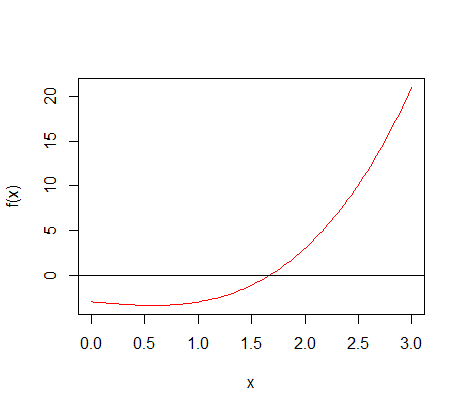
\includegraphics{graph1}\]

\begin{itemize}
\item
  \textbf{Step 2}: Based on the graph, we start with
  \([a,b] = [1.5, 2.0]\)
\item
  \textbf{Step 3}: To determine the no. of iterations, let
  \(|a - c_{n}| = \epsilon = 0.0001\), then solve for \(n\).
\end{itemize}

\[|a - c_{n}| \le [\frac{1}{2}]^{n} (b - a)\]

\[0.0001 \le [\frac{1}{2}]^{n} (2.0 - 1.5)\]

\[0.0001 \le [\frac{1}{2}]^{n} (0.5)\]

\[\frac{0.0001}{0.5} \le [\frac{1}{2}]^{n}\]

\[0.0002 \le [\frac{1}{2}]^{n}\]

\[\ln  0.0002 \le n \ \ln\ [\frac{1}{2}]\]

\[\frac{\ln  0.0002}{\ln \frac{1}{2}} \le n\]

\[\frac{-8.5171931914162374266547336972793}{-0.69314718055994530941723212145818} \le n\]

\[12.28771238 \le n\]

\[n \ge 13\]

\begin{itemize}
\tightlist
\item
  \textbf{Step 4}: The following table is generated starting with
  \(Bisect(f(x) = x^{3} - x - 3, 1.5, 2.0, c_{1}, \epsilon = 0.0001)\).
\end{itemize}

\[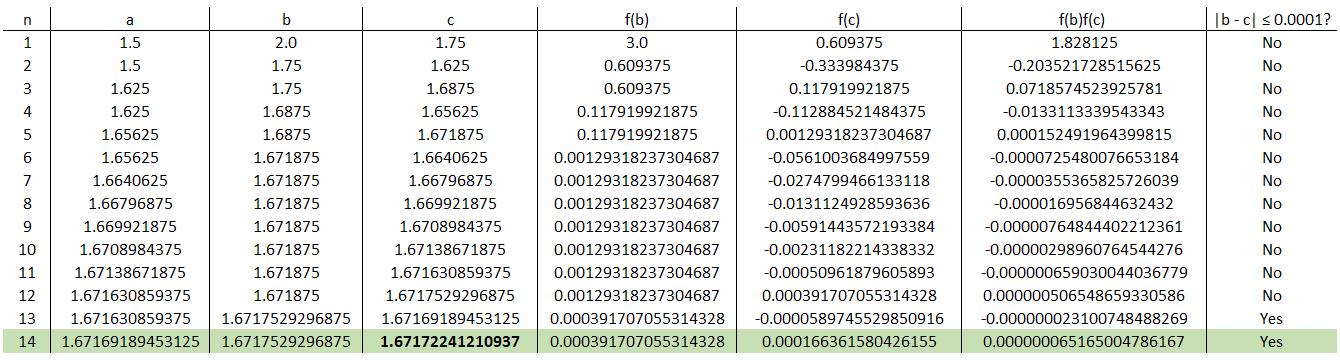
\includegraphics{bisection_table}\]

\begin{itemize}
\tightlist
\item
  \textbf{To conclude}, the real root of the function
  \(f(x) = x^{3} - x - 3\) is \(\colorbox{green}{1.67172241210937}\).
\end{itemize}

\(\textcolor{blue}{2.}\) The function
\(f(x) = -3x^{3} + 2e^{\frac{x^{2}}{2}} - 1\) has values of zero near
\(x = -0.5\) and \(x = 0.5\).

\(\textcolor{blue}{a.}\) What is the derivative of \(f\)?

\[f(x) = -9x^{2} + 2xe^{\frac{x^{2}}{2}}\]

\(\textcolor{blue}{b.}\) If you begin Newton's method at \(x = 0\),
which root is reached? How many iterations to achieve an error less than
\(10^{-5}\)?

\par

Using x = 0, the root is not reached, instead it approaches negative
infinity. To work around this, we used x = 0.2 instead. The root reached
is 0.85679 with a tolerance of 0.000001. It takes nine iterations to
reach the root.

\[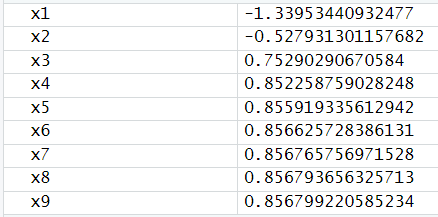
\includegraphics{newton_table}\]

\(\textcolor{blue}{c.}\) Begin Newton's method at another starting point
to get the other zero.

\par

Using x = 0.5. The root reached is 0.85680 with a tolerance of 0.000001.
It takes ten iterations to reach the root.

\[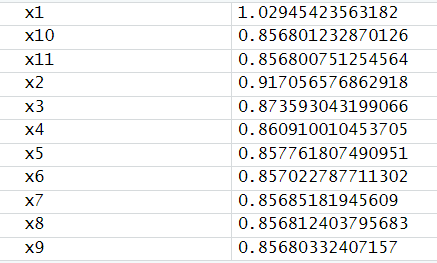
\includegraphics{newton_table3}\]

\(\textcolor{blue}{3.}\) Use the function from no.2 and find the root
using the secant method where \(x_{0} = 0\) and \(x_{1} = 1\). Use an
error tolerance of \(\epsilon = 0.001\).

\begin{itemize}
\tightlist
\item
  \textbf{Step 1}: The graph below is generated using R, and illustrates
  the function \(-3x^3 + 2e^\frac{x^2}{2} - 1\), starting from
  \(x_{0} = 0\) to \(x_{1} = 1\):
\end{itemize}

\[\includegraphics{graph2}\]

\begin{itemize}
\item
  \textbf{Step 2}: Use the general iterative formula for the secant
  method
  \(x_{n+1} = x_{n}-f(x_{n}) \ \cdot \ \frac{x_{n} - x_{n-1}}{f(x_{n})-f(x_{n-1})}\)
  to solve for the root.
\item
  \textbf{Step 2a}: 1st iteration (\(n = 1\), \(x_{n} = 1\),
  \(x_{n-1} = 0\)):
\end{itemize}

\[x_{n+1} = x_{n}-f(x_{n}) \ \cdot \ \frac{x_{n} - x_{n-1}}{f(x_{n})-f(x_{n-1})}\]

\[x_{2} = 1-f(1) \ \cdot \ \frac{1 - 0}{f(1)-f(0)}\]

\[x_{2} = 1 - (-0.7025575) \ \cdot \ \frac{1 - 0}{-0.7025575 - 1}\]

\[x_{2} = 0.587351689629578\]

\begin{itemize}
\tightlist
\item
  \textbf{Step 2b}: 2nd iteration (\(n = 2\),
  \(x_{n} = 0.587351689629578\), \(x_{n-1} = 1\)):
\end{itemize}

\[x_{3} = x_{2}-f(x_{2}) \ \cdot \ \frac{x_{2} - x_{2-1}}{f(x_{2})-f(x_{2-1})}\]

\[x_{3} = 0.802944079420674\]

\begin{itemize}
\tightlist
\item
  \textbf{Step 2c}: 3rd iteration (\(n = 3\),
  \(x_{n} = 0.802944079420674\), \(x_{n-1} = 0.587351689629578\)):
\end{itemize}

\[x_{3+1} = x_{3}-f(x_{3}) \ \cdot \ \frac{x_{3} - x_{3-1}}{f(x_{3})-f(x_{3-1})}\]

\[x_{4} = 0.882793045552439\]

\begin{itemize}
\tightlist
\item
  \textbf{Step 2d}: 4th iteration (\(n = 4\),
  \(x_{n} = 0.882793045552439\), \(x_{n-1} = 0.802944079420674\)):
\end{itemize}

\[x_{4+1} = x_{4}-f(x_{4}) \ \cdot \ \frac{x_{4} - x_{4-1}}{f(x_{4})-f(x_{4-1})}\]

\[x_{5} = 0.854989104029943\]

\begin{itemize}
\tightlist
\item
  \textbf{Step 2e}: 5th iteration (\(n = 5\),
  \(x_{n} = 0.854989104029943\), \(x_{n-1} = 0.882793045552439\)):
\end{itemize}

\[x_{5+1} = x_{5}-f(x_{5}) \ \cdot \ \frac{x_{5} - x_{5-1}}{f(x_{5})-f(x_{5-1})}\]

\[x_{6} = 0.856742662921425\]

\begin{itemize}
\tightlist
\item
  \textbf{Step 2f}: 6th iteration (\(n = 6\),
  \(x_{n} = 0.856742662921425\), \(x_{n-1} = 0.854989104029943\)):
\end{itemize}

\[x_{6+1} = x_{6}-f(x_{6}) \ \cdot \ \frac{x_{6} - x_{6-1}}{f(x_{6})-f(x_{6-1})}\]

\[x_{7} = 0.856800739647502\]

\(\textcolor{blue}{4.}\) Consider the system

\[10.2x + 2.4y - 4.5z = 14.067,\]

\[-2.3x - 7.7y + 11.1z = -0.996,\]

\[-5.5x - 3.2x + 0.9z = -12.645.\]

\(\textcolor{blue}{a.}\) Present the augmented matrix of the system.

\[
  \begin{pmatrix}
    10.2 & 2.4 & -4.5  &\bigm| & 14.067 \\
    -2.3 & -7.7 & 11.1  &\bigm| & -0.996 \\
    -5.5 & -3.2 & 0.9  &\bigm| & -12.645 
  \end{pmatrix}
  \]

\(\textcolor{blue}{b.}\) Solve the system using
\(A_{x} = LU_{x} = L_{y} = b\) and round the final answer to 4 decimal
digits.

\begin{itemize}
\tightlist
\item
  \textbf{Step 1}: Determine the LU matrices first.
\end{itemize}

\[A = LU\]

\[A = 
  \begin{pmatrix}
    1 & 0 & 0 \\
    * & 1 & 0 \\
    * & * & 1 
   \end{pmatrix}
   \begin{pmatrix}
    10.2 & 2.4 & -4.5  &\bigm| & 14.067 \\
    -2.3 & -7.7 & 11.1  &\bigm| & -0.996 \\
    -5.5 & -3.2 & 0.9  &\bigm| & -12.645 
   \end{pmatrix}
   \]

\[
   L = 
   \begin{pmatrix}
    1 & 0 & 0 \\
    * & 1 & 0 \\
    * & * & 1 
   \end{pmatrix}
   \]

\[
   U =
   \begin{pmatrix}
    10.2 & 2.4 & -4.5  &\bigm| & 14.067 \\
    -2.3 & -7.7 & 11.1  &\bigm| & -0.996 \\
    -5.5 & -3.2 & 0.9  &\bigm| & -12.645 
   \end{pmatrix}
   \]

\begin{itemize}
\tightlist
\item
  Row operation:
  \(-0.22549019607843137254901960784314R_{1} - R_{2} \rightarrow R_{2}\)
\end{itemize}

\[
   L = 
   \begin{pmatrix}
    1 & 0 & 0 \\
    -0.22549019607843137254901960784314 & 1 & 0 \\
    * & * & 1 
   \end{pmatrix}
   \]

\[
   U =
   \begin{pmatrix}
    10.2 & 2.4 & -4.5  &\bigm| & 14.067 \\
    0 & -7.15882352941 & 10.0852941  &\bigm| & 2.1759705882352941 \\
    -5.5 & -3.2 & 0.9  &\bigm| & -12.645 
    \end{pmatrix}
   \]

\begin{itemize}
\tightlist
\item
  Row operation:
  \(-0.53921568627450980392156862745098R_{1} - R_{3} \rightarrow R_{3}\)
\end{itemize}

\[
   L = 
   \begin{pmatrix}
    1 & 0 & 0 \\
    -0.22549019607843137254901960784314 & 1 & 0 \\
    -0.53921568627450980392156862745098 & * & 1 
   \end{pmatrix}
   \]

\[
   U =
   \begin{pmatrix}
    10.2 & 2.4 & -4.5  &\bigm| & 14.067 \\
    0 & -7.15882352941 & 10.0852941  &\bigm| & 2.1759705882352941 \\
    0 & -1.90588235294117647 & -1.5264705882352941  &\bigm| & -5.05985294117647 
    \end{pmatrix}
   \]

\begin{itemize}
\tightlist
\item
  Row operation:
  \(0.26622843056696795398520953163516R_{2} - R_{3} \rightarrow R_{3}\)
\end{itemize}

\[
   L = 
   \begin{pmatrix}
    1 & 0 & 0 \\
    -0.22549019607843137254901960784314 & 1 & 0 \\
    -0.53921568627450980392156862745098 & 0.26622843056696795398520953163516 & 1 
   \end{pmatrix}
   \]

\[
   U =
   \begin{pmatrix}
    10.2 & 2.4 & -4.5  &\bigm| & 14.067 \\
    0 & -7.15882352941 & 10.0852941  &\bigm| & 2.1759705882352941 \\
    0 & 0 & -4.211462612982744  &\bigm| & 4.4805477065107 
    \end{pmatrix}
   \]

\begin{itemize}
\tightlist
\item
  \textbf{Step 2}: Use matrix \(L\) in the equation \(L_{y} = b\) to
  find \(y\) via forward substitution.
\end{itemize}

\[L_{y} = b\] \[
   L = 
   \begin{pmatrix}
    1 & 0 & 0 \\
    -0.22549019607843137254901960784314 & 1 & 0 \\
    -0.53921568627450980392156862745098 & 0.26622843056696795398520953163516 & 1 
   \end{pmatrix}
   \] \[
   y = 
   \begin{pmatrix}
    y_{1} \\
    y_{2} \\
    y_{3} 
   \end{pmatrix}
   ,
   b = 
   \begin{pmatrix}
    14.067 \\
    -0.996 \\
    -12.645 
   \end{pmatrix}
   \]

\begin{itemize}
\tightlist
\item
  Solving for \(y_{1}\)
\end{itemize}

\[y_{1} = 14.067\]

\begin{itemize}
\tightlist
\item
  Solving for \(y_{2}\)
\end{itemize}

\[-0.22549019607843137254901960784314y_{1} + y_{2} = -0.996\]
\[y_{2} = 2.1759705882352941176470588235295\]

\begin{itemize}
\tightlist
\item
  Solving for \(y_{3}\)
\end{itemize}

\[-0.53921568627450980392156862745098y_{1} + 0.26622843056696795398520953163516y_{2} + y_{3} = -12.645\]
\[y_{3} = -5.6391581758422350041084634346755\]

\begin{itemize}
\tightlist
\item
  Therefore:
\end{itemize}

\[
    y = 
    \begin{pmatrix}
      y_{1} \\
      y_{2} \\
      y_{3} 
    \end{pmatrix}
    = 
    \begin{pmatrix}
      14.067 \\
      2.1759705882352941176470588235295 \\
      -5.6391581758422350041084634346755 
    \end{pmatrix}
   \]

\begin{itemize}
\tightlist
\item
  \textbf{Step 3}: Use matrix \(U\) and \(y\) from Step 2 in the
  equation \(U_{x} = y\) to find \(x\) via back substitution.
\end{itemize}

\[
   U =
   \begin{pmatrix}
    10.2 & 2.4 & -4.5  &\bigm| & 14.067 \\
    0 & -7.15882352941 & 10.0852941  &\bigm| & 2.1759705882352941 \\
    0 & 0 & -4.211462612982744  &\bigm| & 4.4805477065107 
    \end{pmatrix}
   \] \[
   x = 
   \begin{pmatrix}
    x_{1} \\
    x_{2} \\
    x_{3} 
   \end{pmatrix}
   ,
   y = 
   \begin{pmatrix}
      14.067 \\
      2.1759705882352941176470588235295 \\
      -5.6391581758422350041084634346755 
    \end{pmatrix}
   \]

\begin{itemize}
\tightlist
\item
  Solving for \(x_{3}\)
\end{itemize}

\[-4.211462612982744x_{3} = -5.6391581758422350041084634346755\]
\[x_{3} = 1.3390023120372267259796891919576\]

\begin{itemize}
\tightlist
\item
  Solving for \(x_{2}\)
\end{itemize}

\[-7.1588235294117647...x_{2} + 10.085294117647...x_{3} = 2.175970588235294117647...\]
\[x_{2} = 1.5824194445257397055810822675525\]

\begin{itemize}
\tightlist
\item
  Solving for \(x_{1}\)
\end{itemize}

\[10.2x_{1} + 2.4x_{2} -4.5x_{3} = 14.067\]
\[x_{1} = 1.5975199742456612719131376393807\]

\begin{itemize}
\tightlist
\item
  Therefore:
\end{itemize}

\[
    x = 
    \begin{pmatrix}
      x_{1} \\
      x_{2} \\
      x_{3} 
    \end{pmatrix}
    = 
    \begin{pmatrix}
      1.5975199742456612719131376393807 \\
      1.5824194445257397055810822675525 \\
      1.3390023120372267259796891919576
    \end{pmatrix}
    \approx
    \begin{pmatrix}
      1.5976 \\
      1.5824 \\
      1.3390 
    \end{pmatrix}
   \]

\begin{itemize}
\tightlist
\item
  \textbf{To conclude}, the solution of matrix \(A\) is
  \(x = (1.5976, 1.5824, 1.3390)^{T}\).
\end{itemize}

\(\textcolor{blue}{c.}\) Find the residual vector if the correct
solution is \(x = 1.4531001\), \(y = -1.5891949\), \(z = -0.2748947\).

\begin{itemize}
\tightlist
\item
  \textbf{Step 1}: The following are given values of the variables
  \(b\), \(A\), and \(\bar{x}\):
\end{itemize}

\[
  A = 
  \begin{pmatrix}
    10.2 & 2.4 & -4.5\\
    -2.3 & -7.7 & 11.1\\
    -5.5 & -3.2 & 0.9 
  \end{pmatrix}
  \]

\[
  b = 
  \begin{pmatrix}
    14.067 \\
    -0.996 \\
    -12.645 
  \end{pmatrix}
  \]

\[
  \bar{x} = 
  \begin{pmatrix}
    1.4531001 \\
    -1.5891949 \\
    -0.2748947 
  \end{pmatrix}
  \]

\begin{itemize}
\tightlist
\item
  \textbf{Step 2}: Use the equation \(r = b - A\bar{x}\) to calculate
  the residual error:
\end{itemize}

\[r = b - A\bar{x}\]

\[r = 
  \begin{pmatrix}
    14.067 \\
    -0.996 \\
    -12.645 
  \end{pmatrix}
  -
  \begin{pmatrix}
    10.2 & 2.4 & -4.5\\
    -2.3 & -7.7 & 11.1\\
    -5.5 & -3.2 & 0.9 
  \end{pmatrix}
  \begin{pmatrix}
    1.4531001 \\
    -1.5891949 \\
    -0.2748947 
  \end{pmatrix}\]

\[r = 
  \begin{pmatrix}
    14.067 \\
    -0.996 \\
    -12.645 
  \end{pmatrix}
  -
  \begin{pmatrix}
    10.2(1.4531001) \ \ + & 2.4(-1.5891949) \ \ -  & 4.5(-0.2748947)\\
    -2.3(1.4531001) \ \ + & -7.7(-1.5891949) \ \ +  & 11.1(-0.2748947)\\
    -5.5(1.4531001) \ \ + & -3.2(-1.5891949) \ \ +  & 0.9(-0.2748947) 
  \end{pmatrix}\]

\[r = 
  \begin{pmatrix}
    14.067 \\
    -0.996 \\
    -12.645 
  \end{pmatrix}
  -
  \begin{pmatrix}
    12.24457941\\
    5.84333933\\
    -3.1540321 
  \end{pmatrix}\]

\[r = 
  \begin{pmatrix}
    14.067 - 12.24457941 \\
    -0.996 - 5.84333933\\
    -12.645 +3.1540321
  \end{pmatrix}
  \]

\[r = 
  \begin{pmatrix}
    1.82242059 \\
    -6.83933933\\
    -9.4909679
  \end{pmatrix}
  \]

\begin{itemize}
\tightlist
\item
  \textbf{To conclude}, the residual vector of the solution
  \(x = 1.4531001, y = -1.5891949, z = -0.2748947\) is
  \(r = (1.82242059,-6.83933933,-9.4909679)^{T}\).
\end{itemize}

\(\textcolor{blue}{5.}\) Compute the Frobenius norm, maximum column sum,
and maximum row sum of the matrix:

\[
\begin{pmatrix}
10.2 & 2.4 & 4.5\\
-2.3 & 7.7 & 11.1\\
-5.5 & -3.2 & 0.9
\end{pmatrix}
\] The Frobenius norm is defined as the square root of the sum of the
squares of all the matrix elements.

\begin{itemize}
\tightlist
\item
  \textbf{Step 1}: Solving for the Frobenius norm of the given matrix:
\end{itemize}

\[||A||_f = \sqrt{10.2^2 + 2.4^2 + 4.5^2 + -2.3^2 + 7.7^2 + 11.1^2 + -5.5^2 + -3.2^2 + 0.9^2}\]
\[||A||_f = \sqrt{104.04 + 5.76 + 20.25 + 5.29 + 59.29 + 123.21 + 30.25 + 10.24 + 0.81}\]
\[||A||_f = \sqrt{359.14}\] \[||A||_f = 18.9509894201\]

\begin{itemize}
\item
  \textbf{Step 2}: Solving for the maximum column sum:
\item
  \textbf{Step 2a}: Getting the maximum column sum for column 1:
\end{itemize}

\[
    ||A||_{1}= |10.2| + |-2.3| + |-5.5|
  \] \[
    ||A||_{1}= 18
  \]

\begin{itemize}
\tightlist
\item
  \textbf{Step 2b}: Getting the maximum column sum for column 2:
\end{itemize}

\[
    ||A||_{1}= |2.4| + |7.7| + |-3.2|
  \] \[
    ||A||_{1}= 13.3
  \]

\begin{itemize}
\tightlist
\item
  \textbf{Step 2c}: Getting the maximum column sum for column 3:
\end{itemize}

\[
    ||A||_{1}= |4.5| + |11.1| + |0.9|
  \] \[
    ||A||_{1}= 16.5
  \] * Since column 1 has the highest value, the maximum column sum of A
is \(\colorbox{green}{18}\).

\begin{itemize}
\item
  \textbf{Step 3}: Solving for the maximum row sum:
\item
  \textbf{Step 3a}: Getting the maximum row sum for row 1:
\end{itemize}

\[
    ||A||_{\infty}= |10.2| + |2.4| + |4.5|
  \] \[
    ||A||_{\infty}= 17.1
  \]

\begin{itemize}
\tightlist
\item
  \textbf{Step 3b}: Getting the maximum row sum for row 2:
\end{itemize}

\[
    ||A||_{\infty}= |-2.3| + |7.7| + |11.1|
  \] \[
    ||A||_{\infty}= 21.1
  \]

\begin{itemize}
\tightlist
\item
  \textbf{Step 3c}: Getting the maximum row sum for row 3:
\end{itemize}

\[
    ||A||_{\infty}= |-5.5| + |-3.2| + |0.9|
  \] \[
    ||A||_{\infty}= 9.6
  \] * Since row 2 has the highest value, the maximum row sum of A is
\(\colorbox{green}{21.1}\).

\(\textcolor{blue}{6.}\) Solve the system of equations given in no. 4,
starting with the initial vector of \([0,0,0]\):

\(\textcolor{blue}{a.}\) Solve using the Jacobi method with 2-digit
precision

\begin{Shaded}
\begin{Highlighting}[]
\FunctionTok{library}\NormalTok{(matlib)}
\NormalTok{A}\OtherTok{=}\FunctionTok{matrix}\NormalTok{(}\FunctionTok{c}\NormalTok{(}\FloatTok{10.2}\NormalTok{,}\FloatTok{2.4}\NormalTok{,}\SpecialCharTok{{-}}\FloatTok{4.5}\NormalTok{,}\SpecialCharTok{{-}}\FloatTok{2.3}\NormalTok{,}\SpecialCharTok{{-}}\FloatTok{7.7}\NormalTok{,}\FloatTok{11.1}\NormalTok{,}\SpecialCharTok{{-}}\FloatTok{5.5}\NormalTok{,}\SpecialCharTok{{-}}\FloatTok{3.2}\NormalTok{,}\FloatTok{0.9}\NormalTok{), }\AttributeTok{nrow =} \DecValTok{3}\NormalTok{, }\AttributeTok{byrow =}\NormalTok{ T)}
\NormalTok{b}\OtherTok{=}\FunctionTok{matrix}\NormalTok{(}\FunctionTok{c}\NormalTok{(}\FloatTok{14.067}\NormalTok{,}\SpecialCharTok{{-}}\FloatTok{0.996}\NormalTok{,}\SpecialCharTok{{-}}\FloatTok{12.645}\NormalTok{), }\AttributeTok{nrow =} \DecValTok{3}\NormalTok{, }\AttributeTok{byrow =}\NormalTok{ T)}
\FunctionTok{solve}\NormalTok{(A,b)}
\end{Highlighting}
\end{Shaded}

\begin{verbatim}
##          [,1]
## [1,] 1.597520
## [2,] 1.582419
## [3,] 1.339002
\end{verbatim}

\begin{Shaded}
\begin{Highlighting}[]
\NormalTok{  L}\OtherTok{=}\FunctionTok{matrix}\NormalTok{(}\FunctionTok{c}\NormalTok{(}\FloatTok{0.0}\NormalTok{,}\FloatTok{0.0}\NormalTok{,}\FloatTok{0.0}\NormalTok{,}\SpecialCharTok{{-}}\FloatTok{2.3}\NormalTok{,}\FloatTok{0.0}\NormalTok{,}\FloatTok{0.0}\NormalTok{,}\SpecialCharTok{{-}}\FloatTok{5.5}\NormalTok{,}\SpecialCharTok{{-}}\FloatTok{3.2}\NormalTok{,}\FloatTok{0.0}\NormalTok{), }\AttributeTok{nrow =} \DecValTok{3}\NormalTok{, }\AttributeTok{byrow =}\NormalTok{ T)}
\NormalTok{  D}\OtherTok{=}\FunctionTok{matrix}\NormalTok{(}\FunctionTok{c}\NormalTok{(}\FloatTok{10.2}\NormalTok{,}\FloatTok{0.0}\NormalTok{,}\FloatTok{0.0}\NormalTok{,}\FloatTok{0.0}\NormalTok{,}\SpecialCharTok{{-}}\FloatTok{7.7}\NormalTok{,}\FloatTok{0.0}\NormalTok{,}\FloatTok{0.0}\NormalTok{,}\FloatTok{0.0}\NormalTok{,}\FloatTok{0.9}\NormalTok{), }\AttributeTok{nrow =} \DecValTok{3}\NormalTok{, }\AttributeTok{byrow =}\NormalTok{ T)}
\NormalTok{  U}\OtherTok{=}\FunctionTok{matrix}\NormalTok{(}\FunctionTok{c}\NormalTok{(}\FloatTok{0.0}\NormalTok{,}\FloatTok{2.4}\NormalTok{,}\SpecialCharTok{{-}}\FloatTok{4.5}\NormalTok{,}\FloatTok{0.0}\NormalTok{,}\FloatTok{0.0}\NormalTok{,}\FloatTok{11.1}\NormalTok{,}\FloatTok{0.0}\NormalTok{,}\FloatTok{0.0}\NormalTok{,}\FloatTok{0.0}\NormalTok{), }\AttributeTok{nrow =} \DecValTok{3}\NormalTok{, }\AttributeTok{byrow =}\NormalTok{ T)}
\NormalTok{  b}\OtherTok{=}\FunctionTok{matrix}\NormalTok{(}\FunctionTok{c}\NormalTok{(}\FloatTok{14.067}\NormalTok{,}\SpecialCharTok{{-}}\FloatTok{0.996}\NormalTok{,}\SpecialCharTok{{-}}\FloatTok{12.645}\NormalTok{),}\AttributeTok{nrow =} \DecValTok{3}\NormalTok{, }\AttributeTok{byrow =}\NormalTok{ T)}
\NormalTok{  x0}\OtherTok{=}\FunctionTok{matrix}\NormalTok{(}\FunctionTok{c}\NormalTok{(}\DecValTok{0}\NormalTok{,}\DecValTok{0}\NormalTok{,}\DecValTok{0}\NormalTok{), }\AttributeTok{nrow =} \DecValTok{3}\NormalTok{, }\AttributeTok{byrow =}\NormalTok{ T)}
\NormalTok{  x1}\OtherTok{=}\NormalTok{(}\SpecialCharTok{{-}}\FunctionTok{inv}\NormalTok{(D))}\SpecialCharTok{\%*\%}\NormalTok{(L}\SpecialCharTok{+}\NormalTok{U)}\SpecialCharTok{\%*\%}\NormalTok{x0}\SpecialCharTok{+}\FunctionTok{inv}\NormalTok{(D)}\SpecialCharTok{\%*\%}\NormalTok{b}
\NormalTok{  x1}
\end{Highlighting}
\end{Shaded}

\begin{verbatim}
##             [,1]
## [1,]   1.3791177
## [2,]   0.1293506
## [3,] -14.0500000
\end{verbatim}

\begin{Shaded}
\begin{Highlighting}[]
\NormalTok{  d1 }\OtherTok{=} \FunctionTok{inv}\NormalTok{(D)}
\NormalTok{  d1}
\end{Highlighting}
\end{Shaded}

\begin{verbatim}
##            [,1]       [,2]     [,3]
## [1,] 0.09803922  0.0000000 0.000000
## [2,] 0.00000000 -0.1298701 0.000000
## [3,] 0.00000000  0.0000000 1.111111
\end{verbatim}

\begin{Shaded}
\begin{Highlighting}[]
\NormalTok{  L}\OtherTok{=}\FunctionTok{matrix}\NormalTok{(}\FunctionTok{c}\NormalTok{(}\DecValTok{0}\NormalTok{,}\DecValTok{0}\NormalTok{,}\DecValTok{0}\NormalTok{,}\SpecialCharTok{{-}}\FloatTok{2.3}\NormalTok{,}\DecValTok{0}\NormalTok{,}\DecValTok{0}\NormalTok{,}\SpecialCharTok{{-}}\FloatTok{5.5}\NormalTok{,}\SpecialCharTok{{-}}\FloatTok{3.2}\NormalTok{,}\DecValTok{0}\NormalTok{), }\AttributeTok{nrow =} \DecValTok{3}\NormalTok{, }\AttributeTok{byrow =}\NormalTok{ T)}
\NormalTok{  D}\OtherTok{=}\FunctionTok{matrix}\NormalTok{(}\FunctionTok{c}\NormalTok{(}\FloatTok{10.2}\NormalTok{,}\DecValTok{0}\NormalTok{,}\DecValTok{0}\NormalTok{,}\DecValTok{0}\NormalTok{,}\SpecialCharTok{{-}}\FloatTok{7.7}\NormalTok{,}\DecValTok{0}\NormalTok{,}\DecValTok{0}\NormalTok{,}\DecValTok{0}\NormalTok{,}\FloatTok{0.9}\NormalTok{), }\AttributeTok{nrow =} \DecValTok{3}\NormalTok{, }\AttributeTok{byrow =}\NormalTok{ T)}
\NormalTok{  U}\OtherTok{=}\FunctionTok{matrix}\NormalTok{(}\FunctionTok{c}\NormalTok{(}\DecValTok{0}\NormalTok{,}\FloatTok{2.4}\NormalTok{,}\SpecialCharTok{{-}}\FloatTok{4.5}\NormalTok{,}\DecValTok{0}\NormalTok{,}\DecValTok{0}\NormalTok{,}\FloatTok{11.1}\NormalTok{,}\DecValTok{0}\NormalTok{,}\DecValTok{0}\NormalTok{,}\DecValTok{0}\NormalTok{), }\AttributeTok{nrow =} \DecValTok{3}\NormalTok{, }\AttributeTok{byrow =}\NormalTok{ T)}
\NormalTok{  b}\OtherTok{=}\FunctionTok{matrix}\NormalTok{(}\FunctionTok{c}\NormalTok{(}\FloatTok{14.067}\NormalTok{,}\SpecialCharTok{{-}}\FloatTok{0.996}\NormalTok{,}\SpecialCharTok{{-}}\FloatTok{12.645}\NormalTok{),}\AttributeTok{nrow =} \DecValTok{3}\NormalTok{, }\AttributeTok{byrow =}\NormalTok{ T)}
\NormalTok{  x2}\OtherTok{=}\NormalTok{(}\SpecialCharTok{{-}}\FunctionTok{inv}\NormalTok{(D))}\SpecialCharTok{\%*\%}\NormalTok{(L}\SpecialCharTok{+}\NormalTok{U)}\SpecialCharTok{\%*\%}\NormalTok{x1}\SpecialCharTok{+}\FunctionTok{inv}\NormalTok{(D)}\SpecialCharTok{\%*\%}\NormalTok{b}
\NormalTok{  x2}
\end{Highlighting}
\end{Shaded}

\begin{verbatim}
##            [,1]
## [1,]  -4.849847
## [2,] -20.536490
## [3,]  -5.162145
\end{verbatim}

\begin{Shaded}
\begin{Highlighting}[]
\NormalTok{  L}\OtherTok{=}\FunctionTok{matrix}\NormalTok{(}\FunctionTok{c}\NormalTok{(}\DecValTok{0}\NormalTok{,}\DecValTok{0}\NormalTok{,}\DecValTok{0}\NormalTok{,}\SpecialCharTok{{-}}\FloatTok{2.3}\NormalTok{,}\DecValTok{0}\NormalTok{,}\DecValTok{0}\NormalTok{,}\SpecialCharTok{{-}}\FloatTok{5.5}\NormalTok{,}\SpecialCharTok{{-}}\FloatTok{3.2}\NormalTok{,}\DecValTok{0}\NormalTok{), }\AttributeTok{nrow =} \DecValTok{3}\NormalTok{, }\AttributeTok{byrow =}\NormalTok{ T)}
\NormalTok{  D}\OtherTok{=}\FunctionTok{matrix}\NormalTok{(}\FunctionTok{c}\NormalTok{(}\FloatTok{10.2}\NormalTok{,}\DecValTok{0}\NormalTok{,}\DecValTok{0}\NormalTok{,}\DecValTok{0}\NormalTok{,}\SpecialCharTok{{-}}\FloatTok{7.7}\NormalTok{,}\DecValTok{0}\NormalTok{,}\DecValTok{0}\NormalTok{,}\DecValTok{0}\NormalTok{,}\FloatTok{0.9}\NormalTok{), }\AttributeTok{nrow =} \DecValTok{3}\NormalTok{, }\AttributeTok{byrow =}\NormalTok{ T)}
\NormalTok{  U}\OtherTok{=}\FunctionTok{matrix}\NormalTok{(}\FunctionTok{c}\NormalTok{(}\DecValTok{0}\NormalTok{,}\FloatTok{2.4}\NormalTok{,}\SpecialCharTok{{-}}\FloatTok{4.5}\NormalTok{,}\DecValTok{0}\NormalTok{,}\DecValTok{0}\NormalTok{,}\FloatTok{11.1}\NormalTok{,}\DecValTok{0}\NormalTok{,}\DecValTok{0}\NormalTok{,}\DecValTok{0}\NormalTok{), }\AttributeTok{nrow =} \DecValTok{3}\NormalTok{, }\AttributeTok{byrow =}\NormalTok{ T)}
\NormalTok{  b}\OtherTok{=}\FunctionTok{matrix}\NormalTok{(}\FunctionTok{c}\NormalTok{(}\FloatTok{14.067}\NormalTok{,}\SpecialCharTok{{-}}\FloatTok{0.996}\NormalTok{,}\SpecialCharTok{{-}}\FloatTok{12.645}\NormalTok{),}\AttributeTok{nrow =} \DecValTok{3}\NormalTok{, }\AttributeTok{byrow =}\NormalTok{ T)}
\NormalTok{  x3}\OtherTok{=}\NormalTok{(}\SpecialCharTok{{-}}\FunctionTok{inv}\NormalTok{(D))}\SpecialCharTok{\%*\%}\NormalTok{(L}\SpecialCharTok{+}\NormalTok{U)}\SpecialCharTok{\%*\%}\NormalTok{x2}\SpecialCharTok{+}\FunctionTok{inv}\NormalTok{(D)}\SpecialCharTok{\%*\%}\NormalTok{b}
\NormalTok{  x3}
\end{Highlighting}
\end{Shaded}

\begin{verbatim}
##             [,1]
## [1,]    3.933816
## [2,]   -5.863527
## [3,] -116.706586
\end{verbatim}

\begin{Shaded}
\begin{Highlighting}[]
\NormalTok{  L}\OtherTok{=}\FunctionTok{matrix}\NormalTok{(}\FunctionTok{c}\NormalTok{(}\DecValTok{0}\NormalTok{,}\DecValTok{0}\NormalTok{,}\DecValTok{0}\NormalTok{,}\SpecialCharTok{{-}}\FloatTok{2.3}\NormalTok{,}\DecValTok{0}\NormalTok{,}\DecValTok{0}\NormalTok{,}\SpecialCharTok{{-}}\FloatTok{5.5}\NormalTok{,}\SpecialCharTok{{-}}\FloatTok{3.2}\NormalTok{,}\DecValTok{0}\NormalTok{), }\AttributeTok{nrow =} \DecValTok{3}\NormalTok{, }\AttributeTok{byrow =}\NormalTok{ T)}
\NormalTok{  D}\OtherTok{=}\FunctionTok{matrix}\NormalTok{(}\FunctionTok{c}\NormalTok{(}\FloatTok{10.2}\NormalTok{,}\DecValTok{0}\NormalTok{,}\DecValTok{0}\NormalTok{,}\DecValTok{0}\NormalTok{,}\SpecialCharTok{{-}}\FloatTok{7.7}\NormalTok{,}\DecValTok{0}\NormalTok{,}\DecValTok{0}\NormalTok{,}\DecValTok{0}\NormalTok{,}\FloatTok{0.9}\NormalTok{), }\AttributeTok{nrow =} \DecValTok{3}\NormalTok{, }\AttributeTok{byrow =}\NormalTok{ T)}
\NormalTok{  U}\OtherTok{=}\FunctionTok{matrix}\NormalTok{(}\FunctionTok{c}\NormalTok{(}\DecValTok{0}\NormalTok{,}\FloatTok{2.4}\NormalTok{,}\SpecialCharTok{{-}}\FloatTok{4.5}\NormalTok{,}\DecValTok{0}\NormalTok{,}\DecValTok{0}\NormalTok{,}\FloatTok{11.1}\NormalTok{,}\DecValTok{0}\NormalTok{,}\DecValTok{0}\NormalTok{,}\DecValTok{0}\NormalTok{), }\AttributeTok{nrow =} \DecValTok{3}\NormalTok{, }\AttributeTok{byrow =}\NormalTok{ T)}
\NormalTok{  b}\OtherTok{=}\FunctionTok{matrix}\NormalTok{(}\FunctionTok{c}\NormalTok{(}\FloatTok{14.067}\NormalTok{,}\SpecialCharTok{{-}}\FloatTok{0.996}\NormalTok{,}\SpecialCharTok{{-}}\FloatTok{12.645}\NormalTok{),}\AttributeTok{nrow =} \DecValTok{3}\NormalTok{, }\AttributeTok{byrow =}\NormalTok{ T)}
\NormalTok{  x4}\OtherTok{=}\NormalTok{(}\SpecialCharTok{{-}}\FunctionTok{inv}\NormalTok{(D))}\SpecialCharTok{\%*\%}\NormalTok{(L}\SpecialCharTok{+}\NormalTok{U)}\SpecialCharTok{\%*\%}\NormalTok{x3}\SpecialCharTok{+}\FunctionTok{inv}\NormalTok{(D)}\SpecialCharTok{\%*\%}\NormalTok{b}
\NormalTok{  x4}
\end{Highlighting}
\end{Shaded}

\begin{verbatim}
##            [,1]
## [1,]  -48.72943
## [2,] -169.28505
## [3,]  -10.85811
\end{verbatim}

\begin{Shaded}
\begin{Highlighting}[]
\NormalTok{  L}\OtherTok{=}\FunctionTok{matrix}\NormalTok{(}\FunctionTok{c}\NormalTok{(}\DecValTok{0}\NormalTok{,}\DecValTok{0}\NormalTok{,}\DecValTok{0}\NormalTok{,}\SpecialCharTok{{-}}\FloatTok{2.3}\NormalTok{,}\DecValTok{0}\NormalTok{,}\DecValTok{0}\NormalTok{,}\SpecialCharTok{{-}}\FloatTok{5.5}\NormalTok{,}\SpecialCharTok{{-}}\FloatTok{3.2}\NormalTok{,}\DecValTok{0}\NormalTok{), }\AttributeTok{nrow =} \DecValTok{3}\NormalTok{, }\AttributeTok{byrow =}\NormalTok{ T)}
\NormalTok{  D}\OtherTok{=}\FunctionTok{matrix}\NormalTok{(}\FunctionTok{c}\NormalTok{(}\FloatTok{10.2}\NormalTok{,}\DecValTok{0}\NormalTok{,}\DecValTok{0}\NormalTok{,}\DecValTok{0}\NormalTok{,}\SpecialCharTok{{-}}\FloatTok{7.7}\NormalTok{,}\DecValTok{0}\NormalTok{,}\DecValTok{0}\NormalTok{,}\DecValTok{0}\NormalTok{,}\FloatTok{0.9}\NormalTok{), }\AttributeTok{nrow =} \DecValTok{3}\NormalTok{, }\AttributeTok{byrow =}\NormalTok{ T)}
\NormalTok{  U}\OtherTok{=}\FunctionTok{matrix}\NormalTok{(}\FunctionTok{c}\NormalTok{(}\DecValTok{0}\NormalTok{,}\FloatTok{2.4}\NormalTok{,}\SpecialCharTok{{-}}\FloatTok{4.5}\NormalTok{,}\DecValTok{0}\NormalTok{,}\DecValTok{0}\NormalTok{,}\FloatTok{11.1}\NormalTok{,}\DecValTok{0}\NormalTok{,}\DecValTok{0}\NormalTok{,}\DecValTok{0}\NormalTok{), }\AttributeTok{nrow =} \DecValTok{3}\NormalTok{, }\AttributeTok{byrow =}\NormalTok{ T)}
\NormalTok{  b}\OtherTok{=}\FunctionTok{matrix}\NormalTok{(}\FunctionTok{c}\NormalTok{(}\FloatTok{14.067}\NormalTok{,}\SpecialCharTok{{-}}\FloatTok{0.996}\NormalTok{,}\SpecialCharTok{{-}}\FloatTok{12.645}\NormalTok{),}\AttributeTok{nrow =} \DecValTok{3}\NormalTok{, }\AttributeTok{byrow =}\NormalTok{ T)}
\NormalTok{  x5}\OtherTok{=}\NormalTok{(}\SpecialCharTok{{-}}\FunctionTok{inv}\NormalTok{(D))}\SpecialCharTok{\%*\%}\NormalTok{(L}\SpecialCharTok{+}\NormalTok{U)}\SpecialCharTok{\%*\%}\NormalTok{x4}\SpecialCharTok{+}\FunctionTok{inv}\NormalTok{(D)}\SpecialCharTok{\%*\%}\NormalTok{b}
\NormalTok{  x5}
\end{Highlighting}
\end{Shaded}

\begin{verbatim}
##              [,1]
## [1,]   36.4205532
## [2,]   -0.9677051
## [3,] -913.7433666
\end{verbatim}

\begin{Shaded}
\begin{Highlighting}[]
\NormalTok{  L}\OtherTok{=}\FunctionTok{matrix}\NormalTok{(}\FunctionTok{c}\NormalTok{(}\DecValTok{0}\NormalTok{,}\DecValTok{0}\NormalTok{,}\DecValTok{0}\NormalTok{,}\SpecialCharTok{{-}}\FloatTok{2.3}\NormalTok{,}\DecValTok{0}\NormalTok{,}\DecValTok{0}\NormalTok{,}\SpecialCharTok{{-}}\FloatTok{5.5}\NormalTok{,}\SpecialCharTok{{-}}\FloatTok{3.2}\NormalTok{,}\DecValTok{0}\NormalTok{), }\AttributeTok{nrow =} \DecValTok{3}\NormalTok{, }\AttributeTok{byrow =}\NormalTok{ T)}
\NormalTok{  D}\OtherTok{=}\FunctionTok{matrix}\NormalTok{(}\FunctionTok{c}\NormalTok{(}\FloatTok{10.2}\NormalTok{,}\DecValTok{0}\NormalTok{,}\DecValTok{0}\NormalTok{,}\DecValTok{0}\NormalTok{,}\SpecialCharTok{{-}}\FloatTok{7.7}\NormalTok{,}\DecValTok{0}\NormalTok{,}\DecValTok{0}\NormalTok{,}\DecValTok{0}\NormalTok{,}\FloatTok{0.9}\NormalTok{), }\AttributeTok{nrow =} \DecValTok{3}\NormalTok{, }\AttributeTok{byrow =}\NormalTok{ T)}
\NormalTok{  U}\OtherTok{=}\FunctionTok{matrix}\NormalTok{(}\FunctionTok{c}\NormalTok{(}\DecValTok{0}\NormalTok{,}\FloatTok{2.4}\NormalTok{,}\SpecialCharTok{{-}}\FloatTok{4.5}\NormalTok{,}\DecValTok{0}\NormalTok{,}\DecValTok{0}\NormalTok{,}\FloatTok{11.1}\NormalTok{,}\DecValTok{0}\NormalTok{,}\DecValTok{0}\NormalTok{,}\DecValTok{0}\NormalTok{), }\AttributeTok{nrow =} \DecValTok{3}\NormalTok{, }\AttributeTok{byrow =}\NormalTok{ T)}
\NormalTok{  b}\OtherTok{=}\FunctionTok{matrix}\NormalTok{(}\FunctionTok{c}\NormalTok{(}\FloatTok{14.067}\NormalTok{,}\SpecialCharTok{{-}}\FloatTok{0.996}\NormalTok{,}\SpecialCharTok{{-}}\FloatTok{12.645}\NormalTok{),}\AttributeTok{nrow =} \DecValTok{3}\NormalTok{, }\AttributeTok{byrow =}\NormalTok{ T)}
\NormalTok{  x6}\OtherTok{=}\NormalTok{(}\SpecialCharTok{{-}}\FunctionTok{inv}\NormalTok{(D))}\SpecialCharTok{\%*\%}\NormalTok{(L}\SpecialCharTok{+}\NormalTok{U)}\SpecialCharTok{\%*\%}\NormalTok{x5}\SpecialCharTok{+}\FunctionTok{inv}\NormalTok{(D)}\SpecialCharTok{\%*\%}\NormalTok{b}
\NormalTok{  x6}
\end{Highlighting}
\end{Shaded}

\begin{verbatim}
##            [,1]
## [1,]  -401.5153
## [2,] -1327.9640
## [3,]   205.0793
\end{verbatim}

\begin{Shaded}
\begin{Highlighting}[]
\NormalTok{  L}\OtherTok{=}\FunctionTok{matrix}\NormalTok{(}\FunctionTok{c}\NormalTok{(}\DecValTok{0}\NormalTok{,}\DecValTok{0}\NormalTok{,}\DecValTok{0}\NormalTok{,}\SpecialCharTok{{-}}\FloatTok{2.3}\NormalTok{,}\DecValTok{0}\NormalTok{,}\DecValTok{0}\NormalTok{,}\SpecialCharTok{{-}}\FloatTok{5.5}\NormalTok{,}\SpecialCharTok{{-}}\FloatTok{3.2}\NormalTok{,}\DecValTok{0}\NormalTok{), }\AttributeTok{nrow =} \DecValTok{3}\NormalTok{, }\AttributeTok{byrow =}\NormalTok{ T)}
\NormalTok{  D}\OtherTok{=}\FunctionTok{matrix}\NormalTok{(}\FunctionTok{c}\NormalTok{(}\FloatTok{10.2}\NormalTok{,}\DecValTok{0}\NormalTok{,}\DecValTok{0}\NormalTok{,}\DecValTok{0}\NormalTok{,}\SpecialCharTok{{-}}\FloatTok{7.7}\NormalTok{,}\DecValTok{0}\NormalTok{,}\DecValTok{0}\NormalTok{,}\DecValTok{0}\NormalTok{,}\FloatTok{0.9}\NormalTok{), }\AttributeTok{nrow =} \DecValTok{3}\NormalTok{, }\AttributeTok{byrow =}\NormalTok{ T)}
\NormalTok{  U}\OtherTok{=}\FunctionTok{matrix}\NormalTok{(}\FunctionTok{c}\NormalTok{(}\DecValTok{0}\NormalTok{,}\FloatTok{2.4}\NormalTok{,}\SpecialCharTok{{-}}\FloatTok{4.5}\NormalTok{,}\DecValTok{0}\NormalTok{,}\DecValTok{0}\NormalTok{,}\FloatTok{11.1}\NormalTok{,}\DecValTok{0}\NormalTok{,}\DecValTok{0}\NormalTok{,}\DecValTok{0}\NormalTok{), }\AttributeTok{nrow =} \DecValTok{3}\NormalTok{, }\AttributeTok{byrow =}\NormalTok{ T)}
\NormalTok{  b}\OtherTok{=}\FunctionTok{matrix}\NormalTok{(}\FunctionTok{c}\NormalTok{(}\FloatTok{14.067}\NormalTok{,}\SpecialCharTok{{-}}\FloatTok{0.996}\NormalTok{,}\SpecialCharTok{{-}}\FloatTok{12.645}\NormalTok{),}\AttributeTok{nrow =} \DecValTok{3}\NormalTok{, }\AttributeTok{byrow =}\NormalTok{ T)}
\NormalTok{  x7}\OtherTok{=}\NormalTok{(}\SpecialCharTok{{-}}\FunctionTok{inv}\NormalTok{(D))}\SpecialCharTok{\%*\%}\NormalTok{(L}\SpecialCharTok{+}\NormalTok{U)}\SpecialCharTok{\%*\%}\NormalTok{x6}\SpecialCharTok{+}\FunctionTok{inv}\NormalTok{(D)}\SpecialCharTok{\%*\%}\NormalTok{b}
\NormalTok{  x7}
\end{Highlighting}
\end{Shaded}

\begin{verbatim}
##            [,1]
## [1,]   404.3174
## [2,]   415.6963
## [3,] -7189.4042
\end{verbatim}

\begin{Shaded}
\begin{Highlighting}[]
\NormalTok{  L}\OtherTok{=}\FunctionTok{matrix}\NormalTok{(}\FunctionTok{c}\NormalTok{(}\DecValTok{0}\NormalTok{,}\DecValTok{0}\NormalTok{,}\DecValTok{0}\NormalTok{,}\SpecialCharTok{{-}}\FloatTok{2.3}\NormalTok{,}\DecValTok{0}\NormalTok{,}\DecValTok{0}\NormalTok{,}\SpecialCharTok{{-}}\FloatTok{5.5}\NormalTok{,}\SpecialCharTok{{-}}\FloatTok{3.2}\NormalTok{,}\DecValTok{0}\NormalTok{), }\AttributeTok{nrow =} \DecValTok{3}\NormalTok{, }\AttributeTok{byrow =}\NormalTok{ T)}
\NormalTok{  D}\OtherTok{=}\FunctionTok{matrix}\NormalTok{(}\FunctionTok{c}\NormalTok{(}\FloatTok{10.2}\NormalTok{,}\DecValTok{0}\NormalTok{,}\DecValTok{0}\NormalTok{,}\DecValTok{0}\NormalTok{,}\SpecialCharTok{{-}}\FloatTok{7.7}\NormalTok{,}\DecValTok{0}\NormalTok{,}\DecValTok{0}\NormalTok{,}\DecValTok{0}\NormalTok{,}\FloatTok{0.9}\NormalTok{), }\AttributeTok{nrow =} \DecValTok{3}\NormalTok{, }\AttributeTok{byrow =}\NormalTok{ T)}
\NormalTok{  U}\OtherTok{=}\FunctionTok{matrix}\NormalTok{(}\FunctionTok{c}\NormalTok{(}\DecValTok{0}\NormalTok{,}\FloatTok{2.4}\NormalTok{,}\SpecialCharTok{{-}}\FloatTok{4.5}\NormalTok{,}\DecValTok{0}\NormalTok{,}\DecValTok{0}\NormalTok{,}\FloatTok{11.1}\NormalTok{,}\DecValTok{0}\NormalTok{,}\DecValTok{0}\NormalTok{,}\DecValTok{0}\NormalTok{), }\AttributeTok{nrow =} \DecValTok{3}\NormalTok{, }\AttributeTok{byrow =}\NormalTok{ T)}
\NormalTok{  b}\OtherTok{=}\FunctionTok{matrix}\NormalTok{(}\FunctionTok{c}\NormalTok{(}\FloatTok{14.067}\NormalTok{,}\SpecialCharTok{{-}}\FloatTok{0.996}\NormalTok{,}\SpecialCharTok{{-}}\FloatTok{12.645}\NormalTok{),}\AttributeTok{nrow =} \DecValTok{3}\NormalTok{, }\AttributeTok{byrow =}\NormalTok{ T)}
\NormalTok{  x8}\OtherTok{=}\NormalTok{(}\SpecialCharTok{{-}}\FunctionTok{inv}\NormalTok{(D))}\SpecialCharTok{\%*\%}\NormalTok{(L}\SpecialCharTok{+}\NormalTok{U)}\SpecialCharTok{\%*\%}\NormalTok{x7}\SpecialCharTok{+}\FunctionTok{inv}\NormalTok{(D)}\SpecialCharTok{\%*\%}\NormalTok{b}
\NormalTok{  x8}
\end{Highlighting}
\end{Shaded}

\begin{verbatim}
##            [,1]
## [1,]  -3268.228
## [2,] -10484.587
## [3,]   3934.810
\end{verbatim}

\begin{Shaded}
\begin{Highlighting}[]
\NormalTok{  L}\OtherTok{=}\FunctionTok{matrix}\NormalTok{(}\FunctionTok{c}\NormalTok{(}\DecValTok{0}\NormalTok{,}\DecValTok{0}\NormalTok{,}\DecValTok{0}\NormalTok{,}\SpecialCharTok{{-}}\FloatTok{2.3}\NormalTok{,}\DecValTok{0}\NormalTok{,}\DecValTok{0}\NormalTok{,}\SpecialCharTok{{-}}\FloatTok{5.5}\NormalTok{,}\SpecialCharTok{{-}}\FloatTok{3.2}\NormalTok{,}\DecValTok{0}\NormalTok{), }\AttributeTok{nrow =} \DecValTok{3}\NormalTok{, }\AttributeTok{byrow =}\NormalTok{ T)}
\NormalTok{  D}\OtherTok{=}\FunctionTok{matrix}\NormalTok{(}\FunctionTok{c}\NormalTok{(}\FloatTok{10.2}\NormalTok{,}\DecValTok{0}\NormalTok{,}\DecValTok{0}\NormalTok{,}\DecValTok{0}\NormalTok{,}\SpecialCharTok{{-}}\FloatTok{7.7}\NormalTok{,}\DecValTok{0}\NormalTok{,}\DecValTok{0}\NormalTok{,}\DecValTok{0}\NormalTok{,}\FloatTok{0.9}\NormalTok{), }\AttributeTok{nrow =} \DecValTok{3}\NormalTok{, }\AttributeTok{byrow =}\NormalTok{ T)}
\NormalTok{  U}\OtherTok{=}\FunctionTok{matrix}\NormalTok{(}\FunctionTok{c}\NormalTok{(}\DecValTok{0}\NormalTok{,}\FloatTok{2.4}\NormalTok{,}\SpecialCharTok{{-}}\FloatTok{4.5}\NormalTok{,}\DecValTok{0}\NormalTok{,}\DecValTok{0}\NormalTok{,}\FloatTok{11.1}\NormalTok{,}\DecValTok{0}\NormalTok{,}\DecValTok{0}\NormalTok{,}\DecValTok{0}\NormalTok{), }\AttributeTok{nrow =} \DecValTok{3}\NormalTok{, }\AttributeTok{byrow =}\NormalTok{ T)}
\NormalTok{  b}\OtherTok{=}\FunctionTok{matrix}\NormalTok{(}\FunctionTok{c}\NormalTok{(}\FloatTok{14.067}\NormalTok{,}\SpecialCharTok{{-}}\FloatTok{0.996}\NormalTok{,}\SpecialCharTok{{-}}\FloatTok{12.645}\NormalTok{),}\AttributeTok{nrow =} \DecValTok{3}\NormalTok{, }\AttributeTok{byrow =}\NormalTok{ T)}
\NormalTok{  x9}\OtherTok{=}\NormalTok{(}\SpecialCharTok{{-}}\FunctionTok{inv}\NormalTok{(D))}\SpecialCharTok{\%*\%}\NormalTok{(L}\SpecialCharTok{+}\NormalTok{U)}\SpecialCharTok{\%*\%}\NormalTok{x8}\SpecialCharTok{+}\FunctionTok{inv}\NormalTok{(D)}\SpecialCharTok{\%*\%}\NormalTok{b}
\NormalTok{  x9}
\end{Highlighting}
\end{Shaded}

\begin{verbatim}
##            [,1]
## [1,]   4204.287
## [2,]   6648.612
## [3,] -57265.086
\end{verbatim}

\begin{Shaded}
\begin{Highlighting}[]
\NormalTok{  L}\OtherTok{=}\FunctionTok{matrix}\NormalTok{(}\FunctionTok{c}\NormalTok{(}\DecValTok{0}\NormalTok{,}\DecValTok{0}\NormalTok{,}\DecValTok{0}\NormalTok{,}\SpecialCharTok{{-}}\FloatTok{2.3}\NormalTok{,}\DecValTok{0}\NormalTok{,}\DecValTok{0}\NormalTok{,}\SpecialCharTok{{-}}\FloatTok{5.5}\NormalTok{,}\SpecialCharTok{{-}}\FloatTok{3.2}\NormalTok{,}\DecValTok{0}\NormalTok{), }\AttributeTok{nrow =} \DecValTok{3}\NormalTok{, }\AttributeTok{byrow =}\NormalTok{ T)}
\NormalTok{  D}\OtherTok{=}\FunctionTok{matrix}\NormalTok{(}\FunctionTok{c}\NormalTok{(}\FloatTok{10.2}\NormalTok{,}\DecValTok{0}\NormalTok{,}\DecValTok{0}\NormalTok{,}\DecValTok{0}\NormalTok{,}\SpecialCharTok{{-}}\FloatTok{7.7}\NormalTok{,}\DecValTok{0}\NormalTok{,}\DecValTok{0}\NormalTok{,}\DecValTok{0}\NormalTok{,}\FloatTok{0.9}\NormalTok{), }\AttributeTok{nrow =} \DecValTok{3}\NormalTok{, }\AttributeTok{byrow =}\NormalTok{ T)}
\NormalTok{  U}\OtherTok{=}\FunctionTok{matrix}\NormalTok{(}\FunctionTok{c}\NormalTok{(}\DecValTok{0}\NormalTok{,}\FloatTok{2.4}\NormalTok{,}\SpecialCharTok{{-}}\FloatTok{4.5}\NormalTok{,}\DecValTok{0}\NormalTok{,}\DecValTok{0}\NormalTok{,}\FloatTok{11.1}\NormalTok{,}\DecValTok{0}\NormalTok{,}\DecValTok{0}\NormalTok{,}\DecValTok{0}\NormalTok{), }\AttributeTok{nrow =} \DecValTok{3}\NormalTok{, }\AttributeTok{byrow =}\NormalTok{ T)}
\NormalTok{  b}\OtherTok{=}\FunctionTok{matrix}\NormalTok{(}\FunctionTok{c}\NormalTok{(}\FloatTok{14.067}\NormalTok{,}\SpecialCharTok{{-}}\FloatTok{0.996}\NormalTok{,}\SpecialCharTok{{-}}\FloatTok{12.645}\NormalTok{),}\AttributeTok{nrow =} \DecValTok{3}\NormalTok{, }\AttributeTok{byrow =}\NormalTok{ T)}
\NormalTok{  x10}\OtherTok{=}\NormalTok{(}\SpecialCharTok{{-}}\FunctionTok{inv}\NormalTok{(D))}\SpecialCharTok{\%*\%}\NormalTok{(L}\SpecialCharTok{+}\NormalTok{U)}\SpecialCharTok{\%*\%}\NormalTok{x9}\SpecialCharTok{+}\FunctionTok{inv}\NormalTok{(D)}\SpecialCharTok{\%*\%}\NormalTok{b}
\NormalTok{  x10}
\end{Highlighting}
\end{Shaded}

\begin{verbatim}
##           [,1]
## [1,] -26827.01
## [2,] -83806.66
## [3,]  49318.32
\end{verbatim}

\begin{Shaded}
\begin{Highlighting}[]
\NormalTok{  L}\OtherTok{=}\FunctionTok{matrix}\NormalTok{(}\FunctionTok{c}\NormalTok{(}\DecValTok{0}\NormalTok{,}\DecValTok{0}\NormalTok{,}\DecValTok{0}\NormalTok{,}\SpecialCharTok{{-}}\FloatTok{2.3}\NormalTok{,}\DecValTok{0}\NormalTok{,}\DecValTok{0}\NormalTok{,}\SpecialCharTok{{-}}\FloatTok{5.5}\NormalTok{,}\SpecialCharTok{{-}}\FloatTok{3.2}\NormalTok{,}\DecValTok{0}\NormalTok{), }\AttributeTok{nrow =} \DecValTok{3}\NormalTok{, }\AttributeTok{byrow =}\NormalTok{ T)}
\NormalTok{  D}\OtherTok{=}\FunctionTok{matrix}\NormalTok{(}\FunctionTok{c}\NormalTok{(}\FloatTok{10.2}\NormalTok{,}\DecValTok{0}\NormalTok{,}\DecValTok{0}\NormalTok{,}\DecValTok{0}\NormalTok{,}\SpecialCharTok{{-}}\FloatTok{7.7}\NormalTok{,}\DecValTok{0}\NormalTok{,}\DecValTok{0}\NormalTok{,}\DecValTok{0}\NormalTok{,}\FloatTok{0.9}\NormalTok{), }\AttributeTok{nrow =} \DecValTok{3}\NormalTok{, }\AttributeTok{byrow =}\NormalTok{ T)}
\NormalTok{  U}\OtherTok{=}\FunctionTok{matrix}\NormalTok{(}\FunctionTok{c}\NormalTok{(}\DecValTok{0}\NormalTok{,}\FloatTok{2.4}\NormalTok{,}\SpecialCharTok{{-}}\FloatTok{4.5}\NormalTok{,}\DecValTok{0}\NormalTok{,}\DecValTok{0}\NormalTok{,}\FloatTok{11.1}\NormalTok{,}\DecValTok{0}\NormalTok{,}\DecValTok{0}\NormalTok{,}\DecValTok{0}\NormalTok{), }\AttributeTok{nrow =} \DecValTok{3}\NormalTok{, }\AttributeTok{byrow =}\NormalTok{ T)}
\NormalTok{  b}\OtherTok{=}\FunctionTok{matrix}\NormalTok{(}\FunctionTok{c}\NormalTok{(}\FloatTok{14.067}\NormalTok{,}\SpecialCharTok{{-}}\FloatTok{0.996}\NormalTok{,}\SpecialCharTok{{-}}\FloatTok{12.645}\NormalTok{),}\AttributeTok{nrow =} \DecValTok{3}\NormalTok{, }\AttributeTok{byrow =}\NormalTok{ T)}
\NormalTok{  x11}\OtherTok{=}\NormalTok{(}\SpecialCharTok{{-}}\FunctionTok{inv}\NormalTok{(D))}\SpecialCharTok{\%*\%}\NormalTok{(L}\SpecialCharTok{+}\NormalTok{U)}\SpecialCharTok{\%*\%}\NormalTok{x10}\SpecialCharTok{+}\FunctionTok{inv}\NormalTok{(D)}\SpecialCharTok{\%*\%}\NormalTok{b}
\NormalTok{  x11}
\end{Highlighting}
\end{Shaded}

\begin{verbatim}
##            [,1]
## [1,]   41478.68
## [2,]   79108.63
## [3,] -461936.14
\end{verbatim}

\begin{Shaded}
\begin{Highlighting}[]
\NormalTok{  L}\OtherTok{=}\FunctionTok{matrix}\NormalTok{(}\FunctionTok{c}\NormalTok{(}\DecValTok{0}\NormalTok{,}\DecValTok{0}\NormalTok{,}\DecValTok{0}\NormalTok{,}\SpecialCharTok{{-}}\FloatTok{2.3}\NormalTok{,}\DecValTok{0}\NormalTok{,}\DecValTok{0}\NormalTok{,}\SpecialCharTok{{-}}\FloatTok{5.5}\NormalTok{,}\SpecialCharTok{{-}}\FloatTok{3.2}\NormalTok{,}\DecValTok{0}\NormalTok{), }\AttributeTok{nrow =} \DecValTok{3}\NormalTok{, }\AttributeTok{byrow =}\NormalTok{ T)}
\NormalTok{  D}\OtherTok{=}\FunctionTok{matrix}\NormalTok{(}\FunctionTok{c}\NormalTok{(}\FloatTok{10.2}\NormalTok{,}\DecValTok{0}\NormalTok{,}\DecValTok{0}\NormalTok{,}\DecValTok{0}\NormalTok{,}\SpecialCharTok{{-}}\FloatTok{7.7}\NormalTok{,}\DecValTok{0}\NormalTok{,}\DecValTok{0}\NormalTok{,}\DecValTok{0}\NormalTok{,}\FloatTok{0.9}\NormalTok{), }\AttributeTok{nrow =} \DecValTok{3}\NormalTok{, }\AttributeTok{byrow =}\NormalTok{ T)}
\NormalTok{  U}\OtherTok{=}\FunctionTok{matrix}\NormalTok{(}\FunctionTok{c}\NormalTok{(}\DecValTok{0}\NormalTok{,}\FloatTok{2.4}\NormalTok{,}\SpecialCharTok{{-}}\FloatTok{4.5}\NormalTok{,}\DecValTok{0}\NormalTok{,}\DecValTok{0}\NormalTok{,}\FloatTok{11.1}\NormalTok{,}\DecValTok{0}\NormalTok{,}\DecValTok{0}\NormalTok{,}\DecValTok{0}\NormalTok{), }\AttributeTok{nrow =} \DecValTok{3}\NormalTok{, }\AttributeTok{byrow =}\NormalTok{ T)}
\NormalTok{  b}\OtherTok{=}\FunctionTok{matrix}\NormalTok{(}\FunctionTok{c}\NormalTok{(}\FloatTok{14.067}\NormalTok{,}\SpecialCharTok{{-}}\FloatTok{0.996}\NormalTok{,}\SpecialCharTok{{-}}\FloatTok{12.645}\NormalTok{),}\AttributeTok{nrow =} \DecValTok{3}\NormalTok{, }\AttributeTok{byrow =}\NormalTok{ T)}
\NormalTok{  x12}\OtherTok{=}\NormalTok{(}\SpecialCharTok{{-}}\FunctionTok{inv}\NormalTok{(D))}\SpecialCharTok{\%*\%}\NormalTok{(L}\SpecialCharTok{+}\NormalTok{U)}\SpecialCharTok{\%*\%}\NormalTok{x11}\SpecialCharTok{+}\FunctionTok{inv}\NormalTok{(D)}\SpecialCharTok{\%*\%}\NormalTok{b}
\NormalTok{  x12}
\end{Highlighting}
\end{Shaded}

\begin{verbatim}
##           [,1]
## [1,] -222407.8
## [2,] -678297.5
## [3,]  534741.9
\end{verbatim}

\begin{Shaded}
\begin{Highlighting}[]
\NormalTok{  L}\OtherTok{=}\FunctionTok{matrix}\NormalTok{(}\FunctionTok{c}\NormalTok{(}\DecValTok{0}\NormalTok{,}\DecValTok{0}\NormalTok{,}\DecValTok{0}\NormalTok{,}\SpecialCharTok{{-}}\FloatTok{2.3}\NormalTok{,}\DecValTok{0}\NormalTok{,}\DecValTok{0}\NormalTok{,}\SpecialCharTok{{-}}\FloatTok{5.5}\NormalTok{,}\SpecialCharTok{{-}}\FloatTok{3.2}\NormalTok{,}\DecValTok{0}\NormalTok{), }\AttributeTok{nrow =} \DecValTok{3}\NormalTok{, }\AttributeTok{byrow =}\NormalTok{ T)}
\NormalTok{  D}\OtherTok{=}\FunctionTok{matrix}\NormalTok{(}\FunctionTok{c}\NormalTok{(}\FloatTok{10.2}\NormalTok{,}\DecValTok{0}\NormalTok{,}\DecValTok{0}\NormalTok{,}\DecValTok{0}\NormalTok{,}\SpecialCharTok{{-}}\FloatTok{7.7}\NormalTok{,}\DecValTok{0}\NormalTok{,}\DecValTok{0}\NormalTok{,}\DecValTok{0}\NormalTok{,}\FloatTok{0.9}\NormalTok{), }\AttributeTok{nrow =} \DecValTok{3}\NormalTok{, }\AttributeTok{byrow =}\NormalTok{ T)}
\NormalTok{  U}\OtherTok{=}\FunctionTok{matrix}\NormalTok{(}\FunctionTok{c}\NormalTok{(}\DecValTok{0}\NormalTok{,}\FloatTok{2.4}\NormalTok{,}\SpecialCharTok{{-}}\FloatTok{4.5}\NormalTok{,}\DecValTok{0}\NormalTok{,}\DecValTok{0}\NormalTok{,}\FloatTok{11.1}\NormalTok{,}\DecValTok{0}\NormalTok{,}\DecValTok{0}\NormalTok{,}\DecValTok{0}\NormalTok{), }\AttributeTok{nrow =} \DecValTok{3}\NormalTok{, }\AttributeTok{byrow =}\NormalTok{ T)}
\NormalTok{  b}\OtherTok{=}\FunctionTok{matrix}\NormalTok{(}\FunctionTok{c}\NormalTok{(}\FloatTok{14.067}\NormalTok{,}\SpecialCharTok{{-}}\FloatTok{0.996}\NormalTok{,}\SpecialCharTok{{-}}\FloatTok{12.645}\NormalTok{),}\AttributeTok{nrow =} \DecValTok{3}\NormalTok{, }\AttributeTok{byrow =}\NormalTok{ T)}
\NormalTok{  x13}\OtherTok{=}\NormalTok{(}\SpecialCharTok{{-}}\FunctionTok{inv}\NormalTok{(D))}\SpecialCharTok{\%*\%}\NormalTok{(L}\SpecialCharTok{+}\NormalTok{U)}\SpecialCharTok{\%*\%}\NormalTok{x12}\SpecialCharTok{+}\FunctionTok{inv}\NormalTok{(D)}\SpecialCharTok{\%*\%}\NormalTok{b}
\NormalTok{  x13}
\end{Highlighting}
\end{Shaded}

\begin{verbatim}
##            [,1]
## [1,]   395516.4
## [2,]   837295.3
## [3,] -3770897.3
\end{verbatim}

\begin{Shaded}
\begin{Highlighting}[]
\NormalTok{  L}\OtherTok{=}\FunctionTok{matrix}\NormalTok{(}\FunctionTok{c}\NormalTok{(}\DecValTok{0}\NormalTok{,}\DecValTok{0}\NormalTok{,}\DecValTok{0}\NormalTok{,}\SpecialCharTok{{-}}\FloatTok{2.3}\NormalTok{,}\DecValTok{0}\NormalTok{,}\DecValTok{0}\NormalTok{,}\SpecialCharTok{{-}}\FloatTok{5.5}\NormalTok{,}\SpecialCharTok{{-}}\FloatTok{3.2}\NormalTok{,}\DecValTok{0}\NormalTok{), }\AttributeTok{nrow =} \DecValTok{3}\NormalTok{, }\AttributeTok{byrow =}\NormalTok{ T)}
\NormalTok{  D}\OtherTok{=}\FunctionTok{matrix}\NormalTok{(}\FunctionTok{c}\NormalTok{(}\FloatTok{10.2}\NormalTok{,}\DecValTok{0}\NormalTok{,}\DecValTok{0}\NormalTok{,}\DecValTok{0}\NormalTok{,}\SpecialCharTok{{-}}\FloatTok{7.7}\NormalTok{,}\DecValTok{0}\NormalTok{,}\DecValTok{0}\NormalTok{,}\DecValTok{0}\NormalTok{,}\FloatTok{0.9}\NormalTok{), }\AttributeTok{nrow =} \DecValTok{3}\NormalTok{, }\AttributeTok{byrow =}\NormalTok{ T)}
\NormalTok{  U}\OtherTok{=}\FunctionTok{matrix}\NormalTok{(}\FunctionTok{c}\NormalTok{(}\DecValTok{0}\NormalTok{,}\FloatTok{2.4}\NormalTok{,}\SpecialCharTok{{-}}\FloatTok{4.5}\NormalTok{,}\DecValTok{0}\NormalTok{,}\DecValTok{0}\NormalTok{,}\FloatTok{11.1}\NormalTok{,}\DecValTok{0}\NormalTok{,}\DecValTok{0}\NormalTok{,}\DecValTok{0}\NormalTok{), }\AttributeTok{nrow =} \DecValTok{3}\NormalTok{, }\AttributeTok{byrow =}\NormalTok{ T)}
\NormalTok{  b}\OtherTok{=}\FunctionTok{matrix}\NormalTok{(}\FunctionTok{c}\NormalTok{(}\FloatTok{14.067}\NormalTok{,}\SpecialCharTok{{-}}\FloatTok{0.996}\NormalTok{,}\SpecialCharTok{{-}}\FloatTok{12.645}\NormalTok{),}\AttributeTok{nrow =} \DecValTok{3}\NormalTok{, }\AttributeTok{byrow =}\NormalTok{ T)}
\NormalTok{  x14}\OtherTok{=}\NormalTok{(}\SpecialCharTok{{-}}\FunctionTok{inv}\NormalTok{(D))}\SpecialCharTok{\%*\%}\NormalTok{(L}\SpecialCharTok{+}\NormalTok{U)}\SpecialCharTok{\%*\%}\NormalTok{x13}\SpecialCharTok{+}\FunctionTok{inv}\NormalTok{(D)}\SpecialCharTok{\%*\%}\NormalTok{b}
\NormalTok{  x14}
\end{Highlighting}
\end{Shaded}

\begin{verbatim}
##          [,1]
## [1,] -1860641
## [2,] -5554110
## [3,]  5394080
\end{verbatim}

\begin{Shaded}
\begin{Highlighting}[]
\NormalTok{  L}\OtherTok{=}\FunctionTok{matrix}\NormalTok{(}\FunctionTok{c}\NormalTok{(}\DecValTok{0}\NormalTok{,}\DecValTok{0}\NormalTok{,}\DecValTok{0}\NormalTok{,}\SpecialCharTok{{-}}\FloatTok{2.3}\NormalTok{,}\DecValTok{0}\NormalTok{,}\DecValTok{0}\NormalTok{,}\SpecialCharTok{{-}}\FloatTok{5.5}\NormalTok{,}\SpecialCharTok{{-}}\FloatTok{3.2}\NormalTok{,}\DecValTok{0}\NormalTok{), }\AttributeTok{nrow =} \DecValTok{3}\NormalTok{, }\AttributeTok{byrow =}\NormalTok{ T)}
\NormalTok{  D}\OtherTok{=}\FunctionTok{matrix}\NormalTok{(}\FunctionTok{c}\NormalTok{(}\FloatTok{10.2}\NormalTok{,}\DecValTok{0}\NormalTok{,}\DecValTok{0}\NormalTok{,}\DecValTok{0}\NormalTok{,}\SpecialCharTok{{-}}\FloatTok{7.7}\NormalTok{,}\DecValTok{0}\NormalTok{,}\DecValTok{0}\NormalTok{,}\DecValTok{0}\NormalTok{,}\FloatTok{0.9}\NormalTok{), }\AttributeTok{nrow =} \DecValTok{3}\NormalTok{, }\AttributeTok{byrow =}\NormalTok{ T)}
\NormalTok{  U}\OtherTok{=}\FunctionTok{matrix}\NormalTok{(}\FunctionTok{c}\NormalTok{(}\DecValTok{0}\NormalTok{,}\FloatTok{2.4}\NormalTok{,}\SpecialCharTok{{-}}\FloatTok{4.5}\NormalTok{,}\DecValTok{0}\NormalTok{,}\DecValTok{0}\NormalTok{,}\FloatTok{11.1}\NormalTok{,}\DecValTok{0}\NormalTok{,}\DecValTok{0}\NormalTok{,}\DecValTok{0}\NormalTok{), }\AttributeTok{nrow =} \DecValTok{3}\NormalTok{, }\AttributeTok{byrow =}\NormalTok{ T)}
\NormalTok{  b}\OtherTok{=}\FunctionTok{matrix}\NormalTok{(}\FunctionTok{c}\NormalTok{(}\FloatTok{14.067}\NormalTok{,}\SpecialCharTok{{-}}\FloatTok{0.996}\NormalTok{,}\SpecialCharTok{{-}}\FloatTok{12.645}\NormalTok{),}\AttributeTok{nrow =} \DecValTok{3}\NormalTok{, }\AttributeTok{byrow =}\NormalTok{ T)}
\NormalTok{  x15}\OtherTok{=}\NormalTok{(}\SpecialCharTok{{-}}\FunctionTok{inv}\NormalTok{(D))}\SpecialCharTok{\%*\%}\NormalTok{(L}\SpecialCharTok{+}\NormalTok{U)}\SpecialCharTok{\%*\%}\NormalTok{x14}\SpecialCharTok{+}\FunctionTok{inv}\NormalTok{(D)}\SpecialCharTok{\%*\%}\NormalTok{b}
\NormalTok{  x15}
\end{Highlighting}
\end{Shaded}

\begin{verbatim}
##           [,1]
## [1,]   3686592
## [2,]   8331658
## [3,] -31118542
\end{verbatim}

\begin{Shaded}
\begin{Highlighting}[]
\NormalTok{  L}\OtherTok{=}\FunctionTok{matrix}\NormalTok{(}\FunctionTok{c}\NormalTok{(}\DecValTok{0}\NormalTok{,}\DecValTok{0}\NormalTok{,}\DecValTok{0}\NormalTok{,}\SpecialCharTok{{-}}\FloatTok{2.3}\NormalTok{,}\DecValTok{0}\NormalTok{,}\DecValTok{0}\NormalTok{,}\SpecialCharTok{{-}}\FloatTok{5.5}\NormalTok{,}\SpecialCharTok{{-}}\FloatTok{3.2}\NormalTok{,}\DecValTok{0}\NormalTok{), }\AttributeTok{nrow =} \DecValTok{3}\NormalTok{, }\AttributeTok{byrow =}\NormalTok{ T)}
\NormalTok{  D}\OtherTok{=}\FunctionTok{matrix}\NormalTok{(}\FunctionTok{c}\NormalTok{(}\FloatTok{10.2}\NormalTok{,}\DecValTok{0}\NormalTok{,}\DecValTok{0}\NormalTok{,}\DecValTok{0}\NormalTok{,}\SpecialCharTok{{-}}\FloatTok{7.7}\NormalTok{,}\DecValTok{0}\NormalTok{,}\DecValTok{0}\NormalTok{,}\DecValTok{0}\NormalTok{,}\FloatTok{0.9}\NormalTok{), }\AttributeTok{nrow =} \DecValTok{3}\NormalTok{, }\AttributeTok{byrow =}\NormalTok{ T)}
\NormalTok{  U}\OtherTok{=}\FunctionTok{matrix}\NormalTok{(}\FunctionTok{c}\NormalTok{(}\DecValTok{0}\NormalTok{,}\FloatTok{2.4}\NormalTok{,}\SpecialCharTok{{-}}\FloatTok{4.5}\NormalTok{,}\DecValTok{0}\NormalTok{,}\DecValTok{0}\NormalTok{,}\FloatTok{11.1}\NormalTok{,}\DecValTok{0}\NormalTok{,}\DecValTok{0}\NormalTok{,}\DecValTok{0}\NormalTok{), }\AttributeTok{nrow =} \DecValTok{3}\NormalTok{, }\AttributeTok{byrow =}\NormalTok{ T)}
\NormalTok{  b}\OtherTok{=}\FunctionTok{matrix}\NormalTok{(}\FunctionTok{c}\NormalTok{(}\FloatTok{14.067}\NormalTok{,}\SpecialCharTok{{-}}\FloatTok{0.996}\NormalTok{,}\SpecialCharTok{{-}}\FloatTok{12.645}\NormalTok{),}\AttributeTok{nrow =} \DecValTok{3}\NormalTok{, }\AttributeTok{byrow =}\NormalTok{ T)}
\NormalTok{  x16}\OtherTok{=}\NormalTok{(}\SpecialCharTok{{-}}\FunctionTok{inv}\NormalTok{(D))}\SpecialCharTok{\%*\%}\NormalTok{(L}\SpecialCharTok{+}\NormalTok{U)}\SpecialCharTok{\%*\%}\NormalTok{x15}\SpecialCharTok{+}\FunctionTok{inv}\NormalTok{(D)}\SpecialCharTok{\%*\%}\NormalTok{b}
\NormalTok{  x16}
\end{Highlighting}
\end{Shaded}

\begin{verbatim}
##           [,1]
## [1,] -15689158
## [2,] -45960386
## [3,]  52152835
\end{verbatim}

\begin{Shaded}
\begin{Highlighting}[]
\NormalTok{  L}\OtherTok{=}\FunctionTok{matrix}\NormalTok{(}\FunctionTok{c}\NormalTok{(}\DecValTok{0}\NormalTok{,}\DecValTok{0}\NormalTok{,}\DecValTok{0}\NormalTok{,}\SpecialCharTok{{-}}\FloatTok{2.3}\NormalTok{,}\DecValTok{0}\NormalTok{,}\DecValTok{0}\NormalTok{,}\SpecialCharTok{{-}}\FloatTok{5.5}\NormalTok{,}\SpecialCharTok{{-}}\FloatTok{3.2}\NormalTok{,}\DecValTok{0}\NormalTok{), }\AttributeTok{nrow =} \DecValTok{3}\NormalTok{, }\AttributeTok{byrow =}\NormalTok{ T)}
\NormalTok{  D}\OtherTok{=}\FunctionTok{matrix}\NormalTok{(}\FunctionTok{c}\NormalTok{(}\FloatTok{10.2}\NormalTok{,}\DecValTok{0}\NormalTok{,}\DecValTok{0}\NormalTok{,}\DecValTok{0}\NormalTok{,}\SpecialCharTok{{-}}\FloatTok{7.7}\NormalTok{,}\DecValTok{0}\NormalTok{,}\DecValTok{0}\NormalTok{,}\DecValTok{0}\NormalTok{,}\FloatTok{0.9}\NormalTok{), }\AttributeTok{nrow =} \DecValTok{3}\NormalTok{, }\AttributeTok{byrow =}\NormalTok{ T)}
\NormalTok{  U}\OtherTok{=}\FunctionTok{matrix}\NormalTok{(}\FunctionTok{c}\NormalTok{(}\DecValTok{0}\NormalTok{,}\FloatTok{2.4}\NormalTok{,}\SpecialCharTok{{-}}\FloatTok{4.5}\NormalTok{,}\DecValTok{0}\NormalTok{,}\DecValTok{0}\NormalTok{,}\FloatTok{11.1}\NormalTok{,}\DecValTok{0}\NormalTok{,}\DecValTok{0}\NormalTok{,}\DecValTok{0}\NormalTok{), }\AttributeTok{nrow =} \DecValTok{3}\NormalTok{, }\AttributeTok{byrow =}\NormalTok{ T)}
\NormalTok{  b}\OtherTok{=}\FunctionTok{matrix}\NormalTok{(}\FunctionTok{c}\NormalTok{(}\FloatTok{14.067}\NormalTok{,}\SpecialCharTok{{-}}\FloatTok{0.996}\NormalTok{,}\SpecialCharTok{{-}}\FloatTok{12.645}\NormalTok{),}\AttributeTok{nrow =} \DecValTok{3}\NormalTok{, }\AttributeTok{byrow =}\NormalTok{ T)}
\NormalTok{  x17}\OtherTok{=}\NormalTok{(}\SpecialCharTok{{-}}\FunctionTok{inv}\NormalTok{(D))}\SpecialCharTok{\%*\%}\NormalTok{(L}\SpecialCharTok{+}\NormalTok{U)}\SpecialCharTok{\%*\%}\NormalTok{x16}\SpecialCharTok{+}\FunctionTok{inv}\NormalTok{(D)}\SpecialCharTok{\%*\%}\NormalTok{b}
\NormalTok{  x17}
\end{Highlighting}
\end{Shaded}

\begin{verbatim}
##            [,1]
## [1,]   33822815
## [2,]   79867731
## [3,] -259292907
\end{verbatim}

\begin{Shaded}
\begin{Highlighting}[]
\NormalTok{  L}\OtherTok{=}\FunctionTok{matrix}\NormalTok{(}\FunctionTok{c}\NormalTok{(}\DecValTok{0}\NormalTok{,}\DecValTok{0}\NormalTok{,}\DecValTok{0}\NormalTok{,}\SpecialCharTok{{-}}\FloatTok{2.3}\NormalTok{,}\DecValTok{0}\NormalTok{,}\DecValTok{0}\NormalTok{,}\SpecialCharTok{{-}}\FloatTok{5.5}\NormalTok{,}\SpecialCharTok{{-}}\FloatTok{3.2}\NormalTok{,}\DecValTok{0}\NormalTok{), }\AttributeTok{nrow =} \DecValTok{3}\NormalTok{, }\AttributeTok{byrow =}\NormalTok{ T)}
\NormalTok{  D}\OtherTok{=}\FunctionTok{matrix}\NormalTok{(}\FunctionTok{c}\NormalTok{(}\FloatTok{10.2}\NormalTok{,}\DecValTok{0}\NormalTok{,}\DecValTok{0}\NormalTok{,}\DecValTok{0}\NormalTok{,}\SpecialCharTok{{-}}\FloatTok{7.7}\NormalTok{,}\DecValTok{0}\NormalTok{,}\DecValTok{0}\NormalTok{,}\DecValTok{0}\NormalTok{,}\FloatTok{0.9}\NormalTok{), }\AttributeTok{nrow =} \DecValTok{3}\NormalTok{, }\AttributeTok{byrow =}\NormalTok{ T)}
\NormalTok{  U}\OtherTok{=}\FunctionTok{matrix}\NormalTok{(}\FunctionTok{c}\NormalTok{(}\DecValTok{0}\NormalTok{,}\FloatTok{2.4}\NormalTok{,}\SpecialCharTok{{-}}\FloatTok{4.5}\NormalTok{,}\DecValTok{0}\NormalTok{,}\DecValTok{0}\NormalTok{,}\FloatTok{11.1}\NormalTok{,}\DecValTok{0}\NormalTok{,}\DecValTok{0}\NormalTok{,}\DecValTok{0}\NormalTok{), }\AttributeTok{nrow =} \DecValTok{3}\NormalTok{, }\AttributeTok{byrow =}\NormalTok{ T)}
\NormalTok{  b}\OtherTok{=}\FunctionTok{matrix}\NormalTok{(}\FunctionTok{c}\NormalTok{(}\FloatTok{14.067}\NormalTok{,}\SpecialCharTok{{-}}\FloatTok{0.996}\NormalTok{,}\SpecialCharTok{{-}}\FloatTok{12.645}\NormalTok{),}\AttributeTok{nrow =} \DecValTok{3}\NormalTok{, }\AttributeTok{byrow =}\NormalTok{ T)}
\NormalTok{  x18}\OtherTok{=}\NormalTok{(}\SpecialCharTok{{-}}\FunctionTok{inv}\NormalTok{(D))}\SpecialCharTok{\%*\%}\NormalTok{(L}\SpecialCharTok{+}\NormalTok{U)}\SpecialCharTok{\%*\%}\NormalTok{x17}\SpecialCharTok{+}\FunctionTok{inv}\NormalTok{(D)}\SpecialCharTok{\%*\%}\NormalTok{b}
\NormalTok{  x18}
\end{Highlighting}
\end{Shaded}

\begin{verbatim}
##            [,1]
## [1,] -133186341
## [2,] -383888798
## [3,]  490669120
\end{verbatim}

\begin{Shaded}
\begin{Highlighting}[]
\NormalTok{  L}\OtherTok{=}\FunctionTok{matrix}\NormalTok{(}\FunctionTok{c}\NormalTok{(}\DecValTok{0}\NormalTok{,}\DecValTok{0}\NormalTok{,}\DecValTok{0}\NormalTok{,}\SpecialCharTok{{-}}\FloatTok{2.3}\NormalTok{,}\DecValTok{0}\NormalTok{,}\DecValTok{0}\NormalTok{,}\SpecialCharTok{{-}}\FloatTok{5.5}\NormalTok{,}\SpecialCharTok{{-}}\FloatTok{3.2}\NormalTok{,}\DecValTok{0}\NormalTok{), }\AttributeTok{nrow =} \DecValTok{3}\NormalTok{, }\AttributeTok{byrow =}\NormalTok{ T)}
\NormalTok{  D}\OtherTok{=}\FunctionTok{matrix}\NormalTok{(}\FunctionTok{c}\NormalTok{(}\FloatTok{10.2}\NormalTok{,}\DecValTok{0}\NormalTok{,}\DecValTok{0}\NormalTok{,}\DecValTok{0}\NormalTok{,}\SpecialCharTok{{-}}\FloatTok{7.7}\NormalTok{,}\DecValTok{0}\NormalTok{,}\DecValTok{0}\NormalTok{,}\DecValTok{0}\NormalTok{,}\DecValTok{9}\NormalTok{), }\AttributeTok{nrow =} \DecValTok{3}\NormalTok{, }\AttributeTok{byrow =}\NormalTok{ T)}
\NormalTok{  U}\OtherTok{=}\FunctionTok{matrix}\NormalTok{(}\FunctionTok{c}\NormalTok{(}\DecValTok{0}\NormalTok{,}\FloatTok{2.4}\NormalTok{,}\SpecialCharTok{{-}}\FloatTok{4.5}\NormalTok{,}\DecValTok{0}\NormalTok{,}\DecValTok{0}\NormalTok{,}\FloatTok{11.1}\NormalTok{,}\DecValTok{0}\NormalTok{,}\DecValTok{0}\NormalTok{,}\DecValTok{0}\NormalTok{), }\AttributeTok{nrow =} \DecValTok{3}\NormalTok{, }\AttributeTok{byrow =}\NormalTok{ T)}
\NormalTok{  b}\OtherTok{=}\FunctionTok{matrix}\NormalTok{(}\FunctionTok{c}\NormalTok{(}\FloatTok{14.067}\NormalTok{,}\SpecialCharTok{{-}}\FloatTok{0.996}\NormalTok{,}\SpecialCharTok{{-}}\FloatTok{12.645}\NormalTok{),}\AttributeTok{nrow =} \DecValTok{3}\NormalTok{, }\AttributeTok{byrow =}\NormalTok{ T)}
\NormalTok{  x19}\OtherTok{=}\NormalTok{(}\SpecialCharTok{{-}}\FunctionTok{inv}\NormalTok{(D))}\SpecialCharTok{\%*\%}\NormalTok{(L}\SpecialCharTok{+}\NormalTok{U)}\SpecialCharTok{\%*\%}\NormalTok{x18}\SpecialCharTok{+}\FunctionTok{inv}\NormalTok{(D)}\SpecialCharTok{\%*\%}\NormalTok{b}
\NormalTok{  x19}
\end{Highlighting}
\end{Shaded}

\begin{verbatim}
##            [,1]
## [1,]  306798461
## [2,]  747111145
## [3,] -217885447
\end{verbatim}

\begin{Shaded}
\begin{Highlighting}[]
\NormalTok{  L}\OtherTok{=}\FunctionTok{matrix}\NormalTok{(}\FunctionTok{c}\NormalTok{(}\DecValTok{0}\NormalTok{,}\DecValTok{0}\NormalTok{,}\DecValTok{0}\NormalTok{,}\SpecialCharTok{{-}}\FloatTok{2.3}\NormalTok{,}\DecValTok{0}\NormalTok{,}\DecValTok{0}\NormalTok{,}\SpecialCharTok{{-}}\FloatTok{5.5}\NormalTok{,}\SpecialCharTok{{-}}\FloatTok{3.2}\NormalTok{,}\DecValTok{0}\NormalTok{), }\AttributeTok{nrow =} \DecValTok{3}\NormalTok{, }\AttributeTok{byrow =}\NormalTok{ T)}
\NormalTok{  D}\OtherTok{=}\FunctionTok{matrix}\NormalTok{(}\FunctionTok{c}\NormalTok{(}\FloatTok{10.2}\NormalTok{,}\DecValTok{0}\NormalTok{,}\DecValTok{0}\NormalTok{,}\DecValTok{0}\NormalTok{,}\SpecialCharTok{{-}}\FloatTok{7.7}\NormalTok{,}\DecValTok{0}\NormalTok{,}\DecValTok{0}\NormalTok{,}\DecValTok{0}\NormalTok{,}\DecValTok{9}\NormalTok{), }\AttributeTok{nrow =} \DecValTok{3}\NormalTok{, }\AttributeTok{byrow =}\NormalTok{ T)}
\NormalTok{  U}\OtherTok{=}\FunctionTok{matrix}\NormalTok{(}\FunctionTok{c}\NormalTok{(}\DecValTok{0}\NormalTok{,}\FloatTok{2.4}\NormalTok{,}\SpecialCharTok{{-}}\FloatTok{4.5}\NormalTok{,}\DecValTok{0}\NormalTok{,}\DecValTok{0}\NormalTok{,}\FloatTok{11.1}\NormalTok{,}\DecValTok{0}\NormalTok{,}\DecValTok{0}\NormalTok{,}\DecValTok{0}\NormalTok{), }\AttributeTok{nrow =} \DecValTok{3}\NormalTok{, }\AttributeTok{byrow =}\NormalTok{ T)}
\NormalTok{  b}\OtherTok{=}\FunctionTok{matrix}\NormalTok{(}\FunctionTok{c}\NormalTok{(}\FloatTok{14.067}\NormalTok{,}\SpecialCharTok{{-}}\FloatTok{0.996}\NormalTok{,}\SpecialCharTok{{-}}\FloatTok{12.645}\NormalTok{),}\AttributeTok{nrow =} \DecValTok{3}\NormalTok{, }\AttributeTok{byrow =}\NormalTok{ T)}
\NormalTok{  x20}\OtherTok{=}\NormalTok{(}\SpecialCharTok{{-}}\FunctionTok{inv}\NormalTok{(D))}\SpecialCharTok{\%*\%}\NormalTok{(L}\SpecialCharTok{+}\NormalTok{U)}\SpecialCharTok{\%*\%}\NormalTok{x19}\SpecialCharTok{+}\FunctionTok{inv}\NormalTok{(D)}\SpecialCharTok{\%*\%}\NormalTok{b}
\NormalTok{  x20}
\end{Highlighting}
\end{Shaded}

\begin{verbatim}
##            [,1]
## [1,] -271916801
## [2,] -405735705
## [3,]  453127461
\end{verbatim}

\(\textcolor{blue}{b.}\) Solve using Gauss-Seidel method with 2-digit
precision.

\begin{Shaded}
\begin{Highlighting}[]
\NormalTok{  L}\OtherTok{=}\FunctionTok{matrix}\NormalTok{(}\FunctionTok{c}\NormalTok{(}\FloatTok{0.0}\NormalTok{,}\FloatTok{0.0}\NormalTok{,}\FloatTok{0.0}\NormalTok{,}\SpecialCharTok{{-}}\FloatTok{2.3}\NormalTok{,}\FloatTok{0.0}\NormalTok{,}\FloatTok{0.0}\NormalTok{,}\SpecialCharTok{{-}}\FloatTok{5.5}\NormalTok{,}\SpecialCharTok{{-}}\FloatTok{3.2}\NormalTok{,}\FloatTok{0.0}\NormalTok{), }\AttributeTok{nrow =} \DecValTok{3}\NormalTok{, }\AttributeTok{byrow =}\NormalTok{ T)}
\NormalTok{  D}\OtherTok{=}\FunctionTok{matrix}\NormalTok{(}\FunctionTok{c}\NormalTok{(}\FloatTok{10.2}\NormalTok{,}\FloatTok{0.0}\NormalTok{,}\FloatTok{0.0}\NormalTok{,}\FloatTok{0.0}\NormalTok{,}\SpecialCharTok{{-}}\FloatTok{7.7}\NormalTok{,}\FloatTok{0.0}\NormalTok{,}\FloatTok{0.0}\NormalTok{,}\FloatTok{0.0}\NormalTok{,}\FloatTok{0.9}\NormalTok{), }\AttributeTok{nrow =} \DecValTok{3}\NormalTok{, }\AttributeTok{byrow =}\NormalTok{ T)}
\NormalTok{  U}\OtherTok{=}\FunctionTok{matrix}\NormalTok{(}\FunctionTok{c}\NormalTok{(}\FloatTok{0.0}\NormalTok{,}\FloatTok{2.4}\NormalTok{,}\SpecialCharTok{{-}}\FloatTok{4.5}\NormalTok{,}\FloatTok{0.0}\NormalTok{,}\FloatTok{0.0}\NormalTok{,}\FloatTok{11.1}\NormalTok{,}\FloatTok{0.0}\NormalTok{,}\FloatTok{0.0}\NormalTok{,}\FloatTok{0.0}\NormalTok{), }\AttributeTok{nrow =} \DecValTok{3}\NormalTok{, }\AttributeTok{byrow =}\NormalTok{ T)}
\NormalTok{  b}\OtherTok{=}\FunctionTok{matrix}\NormalTok{(}\FunctionTok{c}\NormalTok{(}\FloatTok{14.067}\NormalTok{,}\SpecialCharTok{{-}}\FloatTok{0.996}\NormalTok{,}\SpecialCharTok{{-}}\FloatTok{12.645}\NormalTok{),}\AttributeTok{nrow =} \DecValTok{3}\NormalTok{, }\AttributeTok{byrow =}\NormalTok{ T)}
\NormalTok{  x0}\OtherTok{=}\FunctionTok{matrix}\NormalTok{(}\FunctionTok{c}\NormalTok{(}\DecValTok{0}\NormalTok{,}\DecValTok{0}\NormalTok{,}\DecValTok{0}\NormalTok{), }\AttributeTok{nrow =} \DecValTok{3}\NormalTok{, }\AttributeTok{byrow =}\NormalTok{ T)}
\NormalTok{ x1}\OtherTok{=}\NormalTok{(}\SpecialCharTok{{-}}\DecValTok{1}\SpecialCharTok{*}\FunctionTok{inv}\NormalTok{(L}\SpecialCharTok{+}\NormalTok{D))}\SpecialCharTok{\%*\%}\NormalTok{U}\SpecialCharTok{\%*\%}\NormalTok{x0}\SpecialCharTok{+}\FunctionTok{inv}\NormalTok{(L}\SpecialCharTok{+}\NormalTok{D)}\SpecialCharTok{\%*\%}\NormalTok{b}
\NormalTok{x1}
\end{Highlighting}
\end{Shaded}

\begin{verbatim}
##            [,1]
## [1,]  1.3791177
## [2,] -0.2825936
## [3,] -6.6268360
\end{verbatim}

\begin{Shaded}
\begin{Highlighting}[]
\NormalTok{A}\SpecialCharTok{==}\NormalTok{L}\SpecialCharTok{+}\NormalTok{D}\SpecialCharTok{+}\NormalTok{U}
\end{Highlighting}
\end{Shaded}

\begin{verbatim}
##      [,1] [,2] [,3]
## [1,] TRUE TRUE TRUE
## [2,] TRUE TRUE TRUE
## [3,] TRUE TRUE TRUE
\end{verbatim}

\begin{Shaded}
\begin{Highlighting}[]
\NormalTok{  L}\OtherTok{=}\FunctionTok{matrix}\NormalTok{(}\FunctionTok{c}\NormalTok{(}\FloatTok{0.0}\NormalTok{,}\FloatTok{0.0}\NormalTok{,}\FloatTok{0.0}\NormalTok{,}\SpecialCharTok{{-}}\FloatTok{2.3}\NormalTok{,}\FloatTok{0.0}\NormalTok{,}\FloatTok{0.0}\NormalTok{,}\SpecialCharTok{{-}}\FloatTok{5.5}\NormalTok{,}\SpecialCharTok{{-}}\FloatTok{3.2}\NormalTok{,}\FloatTok{0.0}\NormalTok{), }\AttributeTok{nrow =} \DecValTok{3}\NormalTok{, }\AttributeTok{byrow =}\NormalTok{ T)}
\NormalTok{  D}\OtherTok{=}\FunctionTok{matrix}\NormalTok{(}\FunctionTok{c}\NormalTok{(}\FloatTok{10.2}\NormalTok{,}\FloatTok{0.0}\NormalTok{,}\FloatTok{0.0}\NormalTok{,}\FloatTok{0.0}\NormalTok{,}\SpecialCharTok{{-}}\FloatTok{7.7}\NormalTok{,}\FloatTok{0.0}\NormalTok{,}\FloatTok{0.0}\NormalTok{,}\FloatTok{0.0}\NormalTok{,}\FloatTok{0.9}\NormalTok{), }\AttributeTok{nrow =} \DecValTok{3}\NormalTok{, }\AttributeTok{byrow =}\NormalTok{ T)}
\NormalTok{  U}\OtherTok{=}\FunctionTok{matrix}\NormalTok{(}\FunctionTok{c}\NormalTok{(}\FloatTok{0.0}\NormalTok{,}\FloatTok{2.4}\NormalTok{,}\SpecialCharTok{{-}}\FloatTok{4.5}\NormalTok{,}\FloatTok{0.0}\NormalTok{,}\FloatTok{0.0}\NormalTok{,}\FloatTok{11.1}\NormalTok{,}\FloatTok{0.0}\NormalTok{,}\FloatTok{0.0}\NormalTok{,}\FloatTok{0.0}\NormalTok{), }\AttributeTok{nrow =} \DecValTok{3}\NormalTok{, }\AttributeTok{byrow =}\NormalTok{ T)}
\NormalTok{  b}\OtherTok{=}\FunctionTok{matrix}\NormalTok{(}\FunctionTok{c}\NormalTok{(}\FloatTok{14.067}\NormalTok{,}\SpecialCharTok{{-}}\FloatTok{0.996}\NormalTok{,}\SpecialCharTok{{-}}\FloatTok{12.645}\NormalTok{),}\AttributeTok{nrow =} \DecValTok{3}\NormalTok{, }\AttributeTok{byrow =}\NormalTok{ T)}
\NormalTok{  x0}\OtherTok{=}\FunctionTok{matrix}\NormalTok{(}\FunctionTok{c}\NormalTok{(}\DecValTok{0}\NormalTok{,}\DecValTok{0}\NormalTok{,}\DecValTok{0}\NormalTok{), }\AttributeTok{nrow =} \DecValTok{3}\NormalTok{, }\AttributeTok{byrow =}\NormalTok{ T)}
\NormalTok{ x2}\OtherTok{=}\NormalTok{(}\SpecialCharTok{{-}}\DecValTok{1}\SpecialCharTok{*}\FunctionTok{inv}\NormalTok{(L}\SpecialCharTok{+}\NormalTok{D))}\SpecialCharTok{\%*\%}\NormalTok{U}\SpecialCharTok{\%*\%}\NormalTok{x1}\SpecialCharTok{+}\FunctionTok{inv}\NormalTok{(L}\SpecialCharTok{+}\NormalTok{D)}\SpecialCharTok{\%*\%}\NormalTok{b}
\NormalTok{x2}
\end{Highlighting}
\end{Shaded}

\begin{verbatim}
##            [,1]
## [1,]  -1.477994
## [2,]  -8.982142
## [3,] -55.018690
\end{verbatim}

\begin{Shaded}
\begin{Highlighting}[]
\NormalTok{  L}\OtherTok{=}\FunctionTok{matrix}\NormalTok{(}\FunctionTok{c}\NormalTok{(}\FloatTok{0.0}\NormalTok{,}\FloatTok{0.0}\NormalTok{,}\FloatTok{0.0}\NormalTok{,}\SpecialCharTok{{-}}\FloatTok{2.3}\NormalTok{,}\FloatTok{0.0}\NormalTok{,}\FloatTok{0.0}\NormalTok{,}\SpecialCharTok{{-}}\FloatTok{5.5}\NormalTok{,}\SpecialCharTok{{-}}\FloatTok{3.2}\NormalTok{,}\FloatTok{0.0}\NormalTok{), }\AttributeTok{nrow =} \DecValTok{3}\NormalTok{, }\AttributeTok{byrow =}\NormalTok{ T)}
\NormalTok{  D}\OtherTok{=}\FunctionTok{matrix}\NormalTok{(}\FunctionTok{c}\NormalTok{(}\FloatTok{10.2}\NormalTok{,}\FloatTok{0.0}\NormalTok{,}\FloatTok{0.0}\NormalTok{,}\FloatTok{0.0}\NormalTok{,}\SpecialCharTok{{-}}\FloatTok{7.7}\NormalTok{,}\FloatTok{0.0}\NormalTok{,}\FloatTok{0.0}\NormalTok{,}\FloatTok{0.0}\NormalTok{,}\FloatTok{0.9}\NormalTok{), }\AttributeTok{nrow =} \DecValTok{3}\NormalTok{, }\AttributeTok{byrow =}\NormalTok{ T)}
\NormalTok{  U}\OtherTok{=}\FunctionTok{matrix}\NormalTok{(}\FunctionTok{c}\NormalTok{(}\FloatTok{0.0}\NormalTok{,}\FloatTok{2.4}\NormalTok{,}\SpecialCharTok{{-}}\FloatTok{4.5}\NormalTok{,}\FloatTok{0.0}\NormalTok{,}\FloatTok{0.0}\NormalTok{,}\FloatTok{11.1}\NormalTok{,}\FloatTok{0.0}\NormalTok{,}\FloatTok{0.0}\NormalTok{,}\FloatTok{0.0}\NormalTok{), }\AttributeTok{nrow =} \DecValTok{3}\NormalTok{, }\AttributeTok{byrow =}\NormalTok{ T)}
\NormalTok{  b}\OtherTok{=}\FunctionTok{matrix}\NormalTok{(}\FunctionTok{c}\NormalTok{(}\FloatTok{14.067}\NormalTok{,}\SpecialCharTok{{-}}\FloatTok{0.996}\NormalTok{,}\SpecialCharTok{{-}}\FloatTok{12.645}\NormalTok{),}\AttributeTok{nrow =} \DecValTok{3}\NormalTok{, }\AttributeTok{byrow =}\NormalTok{ T)}
\NormalTok{  x0}\OtherTok{=}\FunctionTok{matrix}\NormalTok{(}\FunctionTok{c}\NormalTok{(}\DecValTok{0}\NormalTok{,}\DecValTok{0}\NormalTok{,}\DecValTok{0}\NormalTok{), }\AttributeTok{nrow =} \DecValTok{3}\NormalTok{, }\AttributeTok{byrow =}\NormalTok{ T)}
\NormalTok{ x3}\OtherTok{=}\NormalTok{(}\SpecialCharTok{{-}}\DecValTok{1}\SpecialCharTok{*}\FunctionTok{inv}\NormalTok{(L}\SpecialCharTok{+}\NormalTok{D))}\SpecialCharTok{\%*\%}\NormalTok{U}\SpecialCharTok{\%*\%}\NormalTok{x2}\SpecialCharTok{+}\FunctionTok{inv}\NormalTok{(L}\SpecialCharTok{+}\NormalTok{D)}\SpecialCharTok{\%*\%}\NormalTok{b}
\NormalTok{x3}
\end{Highlighting}
\end{Shaded}

\begin{verbatim}
##            [,1]
## [1,]  -20.78039
## [2,]  -72.97618
## [3,] -400.51211
\end{verbatim}

\begin{Shaded}
\begin{Highlighting}[]
\NormalTok{  L}\OtherTok{=}\FunctionTok{matrix}\NormalTok{(}\FunctionTok{c}\NormalTok{(}\FloatTok{0.0}\NormalTok{,}\FloatTok{0.0}\NormalTok{,}\FloatTok{0.0}\NormalTok{,}\SpecialCharTok{{-}}\FloatTok{2.3}\NormalTok{,}\FloatTok{0.0}\NormalTok{,}\FloatTok{0.0}\NormalTok{,}\SpecialCharTok{{-}}\FloatTok{5.5}\NormalTok{,}\SpecialCharTok{{-}}\FloatTok{3.2}\NormalTok{,}\FloatTok{0.0}\NormalTok{), }\AttributeTok{nrow =} \DecValTok{3}\NormalTok{, }\AttributeTok{byrow =}\NormalTok{ T)}
\NormalTok{  D}\OtherTok{=}\FunctionTok{matrix}\NormalTok{(}\FunctionTok{c}\NormalTok{(}\FloatTok{10.2}\NormalTok{,}\FloatTok{0.0}\NormalTok{,}\FloatTok{0.0}\NormalTok{,}\FloatTok{0.0}\NormalTok{,}\SpecialCharTok{{-}}\FloatTok{7.7}\NormalTok{,}\FloatTok{0.0}\NormalTok{,}\FloatTok{0.0}\NormalTok{,}\FloatTok{0.0}\NormalTok{,}\FloatTok{0.9}\NormalTok{), }\AttributeTok{nrow =} \DecValTok{3}\NormalTok{, }\AttributeTok{byrow =}\NormalTok{ T)}
\NormalTok{  U}\OtherTok{=}\FunctionTok{matrix}\NormalTok{(}\FunctionTok{c}\NormalTok{(}\FloatTok{0.0}\NormalTok{,}\FloatTok{2.4}\NormalTok{,}\SpecialCharTok{{-}}\FloatTok{4.5}\NormalTok{,}\FloatTok{0.0}\NormalTok{,}\FloatTok{0.0}\NormalTok{,}\FloatTok{11.1}\NormalTok{,}\FloatTok{0.0}\NormalTok{,}\FloatTok{0.0}\NormalTok{,}\FloatTok{0.0}\NormalTok{), }\AttributeTok{nrow =} \DecValTok{3}\NormalTok{, }\AttributeTok{byrow =}\NormalTok{ T)}
\NormalTok{  b}\OtherTok{=}\FunctionTok{matrix}\NormalTok{(}\FunctionTok{c}\NormalTok{(}\FloatTok{14.067}\NormalTok{,}\SpecialCharTok{{-}}\FloatTok{0.996}\NormalTok{,}\SpecialCharTok{{-}}\FloatTok{12.645}\NormalTok{),}\AttributeTok{nrow =} \DecValTok{3}\NormalTok{, }\AttributeTok{byrow =}\NormalTok{ T)}
\NormalTok{  x0}\OtherTok{=}\FunctionTok{matrix}\NormalTok{(}\FunctionTok{c}\NormalTok{(}\DecValTok{0}\NormalTok{,}\DecValTok{0}\NormalTok{,}\DecValTok{0}\NormalTok{), }\AttributeTok{nrow =} \DecValTok{3}\NormalTok{, }\AttributeTok{byrow =}\NormalTok{ T)}
\NormalTok{ x4}\OtherTok{=}\NormalTok{(}\SpecialCharTok{{-}}\DecValTok{1}\SpecialCharTok{*}\FunctionTok{inv}\NormalTok{(L}\SpecialCharTok{+}\NormalTok{D))}\SpecialCharTok{\%*\%}\NormalTok{U}\SpecialCharTok{\%*\%}\NormalTok{x3}\SpecialCharTok{+}\FunctionTok{inv}\NormalTok{(L}\SpecialCharTok{+}\NormalTok{D)}\SpecialCharTok{\%*\%}\NormalTok{b}
\NormalTok{x4}
\end{Highlighting}
\end{Shaded}

\begin{verbatim}
##            [,1]
## [1,]  -158.1465
## [2,]  -529.9937
## [3,] -2864.9231
\end{verbatim}

\begin{Shaded}
\begin{Highlighting}[]
\NormalTok{  L}\OtherTok{=}\FunctionTok{matrix}\NormalTok{(}\FunctionTok{c}\NormalTok{(}\FloatTok{0.0}\NormalTok{,}\FloatTok{0.0}\NormalTok{,}\FloatTok{0.0}\NormalTok{,}\SpecialCharTok{{-}}\FloatTok{2.3}\NormalTok{,}\FloatTok{0.0}\NormalTok{,}\FloatTok{0.0}\NormalTok{,}\SpecialCharTok{{-}}\FloatTok{5.5}\NormalTok{,}\SpecialCharTok{{-}}\FloatTok{3.2}\NormalTok{,}\FloatTok{0.0}\NormalTok{), }\AttributeTok{nrow =} \DecValTok{3}\NormalTok{, }\AttributeTok{byrow =}\NormalTok{ T)}
\NormalTok{  D}\OtherTok{=}\FunctionTok{matrix}\NormalTok{(}\FunctionTok{c}\NormalTok{(}\FloatTok{10.2}\NormalTok{,}\FloatTok{0.0}\NormalTok{,}\FloatTok{0.0}\NormalTok{,}\FloatTok{0.0}\NormalTok{,}\SpecialCharTok{{-}}\FloatTok{7.7}\NormalTok{,}\FloatTok{0.0}\NormalTok{,}\FloatTok{0.0}\NormalTok{,}\FloatTok{0.0}\NormalTok{,}\FloatTok{0.9}\NormalTok{), }\AttributeTok{nrow =} \DecValTok{3}\NormalTok{, }\AttributeTok{byrow =}\NormalTok{ T)}
\NormalTok{  U}\OtherTok{=}\FunctionTok{matrix}\NormalTok{(}\FunctionTok{c}\NormalTok{(}\FloatTok{0.0}\NormalTok{,}\FloatTok{2.4}\NormalTok{,}\SpecialCharTok{{-}}\FloatTok{4.5}\NormalTok{,}\FloatTok{0.0}\NormalTok{,}\FloatTok{0.0}\NormalTok{,}\FloatTok{11.1}\NormalTok{,}\FloatTok{0.0}\NormalTok{,}\FloatTok{0.0}\NormalTok{,}\FloatTok{0.0}\NormalTok{), }\AttributeTok{nrow =} \DecValTok{3}\NormalTok{, }\AttributeTok{byrow =}\NormalTok{ T)}
\NormalTok{  b}\OtherTok{=}\FunctionTok{matrix}\NormalTok{(}\FunctionTok{c}\NormalTok{(}\FloatTok{14.067}\NormalTok{,}\SpecialCharTok{{-}}\FloatTok{0.996}\NormalTok{,}\SpecialCharTok{{-}}\FloatTok{12.645}\NormalTok{),}\AttributeTok{nrow =} \DecValTok{3}\NormalTok{, }\AttributeTok{byrow =}\NormalTok{ T)}
\NormalTok{  x0}\OtherTok{=}\FunctionTok{matrix}\NormalTok{(}\FunctionTok{c}\NormalTok{(}\DecValTok{0}\NormalTok{,}\DecValTok{0}\NormalTok{,}\DecValTok{0}\NormalTok{), }\AttributeTok{nrow =} \DecValTok{3}\NormalTok{, }\AttributeTok{byrow =}\NormalTok{ T)}
\NormalTok{  x5}\OtherTok{=}\NormalTok{(}\SpecialCharTok{{-}}\DecValTok{1}\SpecialCharTok{*}\FunctionTok{inv}\NormalTok{(L}\SpecialCharTok{+}\NormalTok{D))}\SpecialCharTok{\%*\%}\NormalTok{U}\SpecialCharTok{\%*\%}\NormalTok{x4}\SpecialCharTok{+}\FunctionTok{inv}\NormalTok{(L}\SpecialCharTok{+}\NormalTok{D)}\SpecialCharTok{\%*\%}\NormalTok{b}
\NormalTok{  x5}
\end{Highlighting}
\end{Shaded}

\begin{verbatim}
##            [,1]
## [1,]  -1137.853
## [2,]  -3789.946
## [3,] -20442.962
\end{verbatim}

\begin{Shaded}
\begin{Highlighting}[]
\NormalTok{  L}\OtherTok{=}\FunctionTok{matrix}\NormalTok{(}\FunctionTok{c}\NormalTok{(}\FloatTok{0.0}\NormalTok{,}\FloatTok{0.0}\NormalTok{,}\FloatTok{0.0}\NormalTok{,}\SpecialCharTok{{-}}\FloatTok{2.3}\NormalTok{,}\FloatTok{0.0}\NormalTok{,}\FloatTok{0.0}\NormalTok{,}\SpecialCharTok{{-}}\FloatTok{5.5}\NormalTok{,}\SpecialCharTok{{-}}\FloatTok{3.2}\NormalTok{,}\FloatTok{0.0}\NormalTok{), }\AttributeTok{nrow =} \DecValTok{3}\NormalTok{, }\AttributeTok{byrow =}\NormalTok{ T)}
\NormalTok{  D}\OtherTok{=}\FunctionTok{matrix}\NormalTok{(}\FunctionTok{c}\NormalTok{(}\FloatTok{10.2}\NormalTok{,}\FloatTok{0.0}\NormalTok{,}\FloatTok{0.0}\NormalTok{,}\FloatTok{0.0}\NormalTok{,}\SpecialCharTok{{-}}\FloatTok{7.7}\NormalTok{,}\FloatTok{0.0}\NormalTok{,}\FloatTok{0.0}\NormalTok{,}\FloatTok{0.0}\NormalTok{,}\FloatTok{0.9}\NormalTok{), }\AttributeTok{nrow =} \DecValTok{3}\NormalTok{, }\AttributeTok{byrow =}\NormalTok{ T)}
\NormalTok{  U}\OtherTok{=}\FunctionTok{matrix}\NormalTok{(}\FunctionTok{c}\NormalTok{(}\FloatTok{0.0}\NormalTok{,}\FloatTok{2.4}\NormalTok{,}\SpecialCharTok{{-}}\FloatTok{4.5}\NormalTok{,}\FloatTok{0.0}\NormalTok{,}\FloatTok{0.0}\NormalTok{,}\FloatTok{11.1}\NormalTok{,}\FloatTok{0.0}\NormalTok{,}\FloatTok{0.0}\NormalTok{,}\FloatTok{0.0}\NormalTok{), }\AttributeTok{nrow =} \DecValTok{3}\NormalTok{, }\AttributeTok{byrow =}\NormalTok{ T)}
\NormalTok{  b}\OtherTok{=}\FunctionTok{matrix}\NormalTok{(}\FunctionTok{c}\NormalTok{(}\FloatTok{14.067}\NormalTok{,}\SpecialCharTok{{-}}\FloatTok{0.996}\NormalTok{,}\SpecialCharTok{{-}}\FloatTok{12.645}\NormalTok{),}\AttributeTok{nrow =} \DecValTok{3}\NormalTok{, }\AttributeTok{byrow =}\NormalTok{ T)}
\NormalTok{  x0}\OtherTok{=}\FunctionTok{matrix}\NormalTok{(}\FunctionTok{c}\NormalTok{(}\DecValTok{0}\NormalTok{,}\DecValTok{0}\NormalTok{,}\DecValTok{0}\NormalTok{), }\AttributeTok{nrow =} \DecValTok{3}\NormalTok{, }\AttributeTok{byrow =}\NormalTok{ T)}
\NormalTok{ x6}\OtherTok{=}\NormalTok{(}\SpecialCharTok{{-}}\DecValTok{1}\SpecialCharTok{*}\FunctionTok{inv}\NormalTok{(L}\SpecialCharTok{+}\NormalTok{D))}\SpecialCharTok{\%*\%}\NormalTok{U}\SpecialCharTok{\%*\%}\NormalTok{x5}\SpecialCharTok{+}\FunctionTok{inv}\NormalTok{(L}\SpecialCharTok{+}\NormalTok{D)}\SpecialCharTok{\%*\%}\NormalTok{b}
\NormalTok{x6}
\end{Highlighting}
\end{Shaded}

\begin{verbatim}
##             [,1]
## [1,]   -8125.823
## [2,]  -27042.402
## [3,] -145822.615
\end{verbatim}

\begin{Shaded}
\begin{Highlighting}[]
\NormalTok{  L}\OtherTok{=}\FunctionTok{matrix}\NormalTok{(}\FunctionTok{c}\NormalTok{(}\FloatTok{0.0}\NormalTok{,}\FloatTok{0.0}\NormalTok{,}\FloatTok{0.0}\NormalTok{,}\SpecialCharTok{{-}}\FloatTok{2.3}\NormalTok{,}\FloatTok{0.0}\NormalTok{,}\FloatTok{0.0}\NormalTok{,}\SpecialCharTok{{-}}\FloatTok{5.5}\NormalTok{,}\SpecialCharTok{{-}}\FloatTok{3.2}\NormalTok{,}\FloatTok{0.0}\NormalTok{), }\AttributeTok{nrow =} \DecValTok{3}\NormalTok{, }\AttributeTok{byrow =}\NormalTok{ T)}
\NormalTok{  D}\OtherTok{=}\FunctionTok{matrix}\NormalTok{(}\FunctionTok{c}\NormalTok{(}\FloatTok{10.2}\NormalTok{,}\FloatTok{0.0}\NormalTok{,}\FloatTok{0.0}\NormalTok{,}\FloatTok{0.0}\NormalTok{,}\SpecialCharTok{{-}}\FloatTok{7.7}\NormalTok{,}\FloatTok{0.0}\NormalTok{,}\FloatTok{0.0}\NormalTok{,}\FloatTok{0.0}\NormalTok{,}\FloatTok{0.9}\NormalTok{), }\AttributeTok{nrow =} \DecValTok{3}\NormalTok{, }\AttributeTok{byrow =}\NormalTok{ T)}
\NormalTok{  U}\OtherTok{=}\FunctionTok{matrix}\NormalTok{(}\FunctionTok{c}\NormalTok{(}\FloatTok{0.0}\NormalTok{,}\FloatTok{2.4}\NormalTok{,}\SpecialCharTok{{-}}\FloatTok{4.5}\NormalTok{,}\FloatTok{0.0}\NormalTok{,}\FloatTok{0.0}\NormalTok{,}\FloatTok{11.1}\NormalTok{,}\FloatTok{0.0}\NormalTok{,}\FloatTok{0.0}\NormalTok{,}\FloatTok{0.0}\NormalTok{), }\AttributeTok{nrow =} \DecValTok{3}\NormalTok{, }\AttributeTok{byrow =}\NormalTok{ T)}
\NormalTok{  b}\OtherTok{=}\FunctionTok{matrix}\NormalTok{(}\FunctionTok{c}\NormalTok{(}\FloatTok{14.067}\NormalTok{,}\SpecialCharTok{{-}}\FloatTok{0.996}\NormalTok{,}\SpecialCharTok{{-}}\FloatTok{12.645}\NormalTok{),}\AttributeTok{nrow =} \DecValTok{3}\NormalTok{, }\AttributeTok{byrow =}\NormalTok{ T)}
\NormalTok{  x0}\OtherTok{=}\FunctionTok{matrix}\NormalTok{(}\FunctionTok{c}\NormalTok{(}\DecValTok{0}\NormalTok{,}\DecValTok{0}\NormalTok{,}\DecValTok{0}\NormalTok{), }\AttributeTok{nrow =} \DecValTok{3}\NormalTok{, }\AttributeTok{byrow =}\NormalTok{ T)}
\NormalTok{ x7}\OtherTok{=}\NormalTok{(}\SpecialCharTok{{-}}\DecValTok{1}\SpecialCharTok{*}\FunctionTok{inv}\NormalTok{(L}\SpecialCharTok{+}\NormalTok{D))}\SpecialCharTok{\%*\%}\NormalTok{U}\SpecialCharTok{\%*\%}\NormalTok{x6}\SpecialCharTok{+}\FunctionTok{inv}\NormalTok{(L}\SpecialCharTok{+}\NormalTok{D)}\SpecialCharTok{\%*\%}\NormalTok{b}
\NormalTok{x7}
\end{Highlighting}
\end{Shaded}

\begin{verbatim}
##             [,1]
## [1,]   -57969.21
## [2,]  -192896.21
## [3,] -1040123.53
\end{verbatim}

\begin{Shaded}
\begin{Highlighting}[]
\NormalTok{  L}\OtherTok{=}\FunctionTok{matrix}\NormalTok{(}\FunctionTok{c}\NormalTok{(}\FloatTok{0.0}\NormalTok{,}\FloatTok{0.0}\NormalTok{,}\FloatTok{0.0}\NormalTok{,}\SpecialCharTok{{-}}\FloatTok{2.3}\NormalTok{,}\FloatTok{0.0}\NormalTok{,}\FloatTok{0.0}\NormalTok{,}\SpecialCharTok{{-}}\FloatTok{5.5}\NormalTok{,}\SpecialCharTok{{-}}\FloatTok{3.2}\NormalTok{,}\FloatTok{0.0}\NormalTok{), }\AttributeTok{nrow =} \DecValTok{3}\NormalTok{, }\AttributeTok{byrow =}\NormalTok{ T)}
\NormalTok{  D}\OtherTok{=}\FunctionTok{matrix}\NormalTok{(}\FunctionTok{c}\NormalTok{(}\FloatTok{10.2}\NormalTok{,}\FloatTok{0.0}\NormalTok{,}\FloatTok{0.0}\NormalTok{,}\FloatTok{0.0}\NormalTok{,}\SpecialCharTok{{-}}\FloatTok{7.7}\NormalTok{,}\FloatTok{0.0}\NormalTok{,}\FloatTok{0.0}\NormalTok{,}\FloatTok{0.0}\NormalTok{,}\FloatTok{0.9}\NormalTok{), }\AttributeTok{nrow =} \DecValTok{3}\NormalTok{, }\AttributeTok{byrow =}\NormalTok{ T)}
\NormalTok{  U}\OtherTok{=}\FunctionTok{matrix}\NormalTok{(}\FunctionTok{c}\NormalTok{(}\FloatTok{0.0}\NormalTok{,}\FloatTok{2.4}\NormalTok{,}\SpecialCharTok{{-}}\FloatTok{4.5}\NormalTok{,}\FloatTok{0.0}\NormalTok{,}\FloatTok{0.0}\NormalTok{,}\FloatTok{11.1}\NormalTok{,}\FloatTok{0.0}\NormalTok{,}\FloatTok{0.0}\NormalTok{,}\FloatTok{0.0}\NormalTok{), }\AttributeTok{nrow =} \DecValTok{3}\NormalTok{, }\AttributeTok{byrow =}\NormalTok{ T)}
\NormalTok{  b}\OtherTok{=}\FunctionTok{matrix}\NormalTok{(}\FunctionTok{c}\NormalTok{(}\FloatTok{14.067}\NormalTok{,}\SpecialCharTok{{-}}\FloatTok{0.996}\NormalTok{,}\SpecialCharTok{{-}}\FloatTok{12.645}\NormalTok{),}\AttributeTok{nrow =} \DecValTok{3}\NormalTok{, }\AttributeTok{byrow =}\NormalTok{ T)}
\NormalTok{  x0}\OtherTok{=}\FunctionTok{matrix}\NormalTok{(}\FunctionTok{c}\NormalTok{(}\DecValTok{0}\NormalTok{,}\DecValTok{0}\NormalTok{,}\DecValTok{0}\NormalTok{), }\AttributeTok{nrow =} \DecValTok{3}\NormalTok{, }\AttributeTok{byrow =}\NormalTok{ T)}
\NormalTok{  x8}\OtherTok{=}\NormalTok{(}\SpecialCharTok{{-}}\DecValTok{1}\SpecialCharTok{*}\FunctionTok{inv}\NormalTok{(L}\SpecialCharTok{+}\NormalTok{D))}\SpecialCharTok{\%*\%}\NormalTok{U}\SpecialCharTok{\%*\%}\NormalTok{x7}\SpecialCharTok{+}\FunctionTok{inv}\NormalTok{(L}\SpecialCharTok{+}\NormalTok{D)}\SpecialCharTok{\%*\%}\NormalTok{b}
\NormalTok{  x8}
\end{Highlighting}
\end{Shaded}

\begin{verbatim}
##            [,1]
## [1,]  -413489.3
## [2,] -1375888.9
## [3,] -7418942.6
\end{verbatim}

\begin{Shaded}
\begin{Highlighting}[]
\NormalTok{  L}\OtherTok{=}\FunctionTok{matrix}\NormalTok{(}\FunctionTok{c}\NormalTok{(}\FloatTok{0.0}\NormalTok{,}\FloatTok{0.0}\NormalTok{,}\FloatTok{0.0}\NormalTok{,}\SpecialCharTok{{-}}\FloatTok{2.3}\NormalTok{,}\FloatTok{0.0}\NormalTok{,}\FloatTok{0.0}\NormalTok{,}\SpecialCharTok{{-}}\FloatTok{5.5}\NormalTok{,}\SpecialCharTok{{-}}\FloatTok{3.2}\NormalTok{,}\FloatTok{0.0}\NormalTok{), }\AttributeTok{nrow =} \DecValTok{3}\NormalTok{, }\AttributeTok{byrow =}\NormalTok{ T)}
\NormalTok{  D}\OtherTok{=}\FunctionTok{matrix}\NormalTok{(}\FunctionTok{c}\NormalTok{(}\FloatTok{10.2}\NormalTok{,}\FloatTok{0.0}\NormalTok{,}\FloatTok{0.0}\NormalTok{,}\FloatTok{0.0}\NormalTok{,}\SpecialCharTok{{-}}\FloatTok{7.7}\NormalTok{,}\FloatTok{0.0}\NormalTok{,}\FloatTok{0.0}\NormalTok{,}\FloatTok{0.0}\NormalTok{,}\FloatTok{0.9}\NormalTok{), }\AttributeTok{nrow =} \DecValTok{3}\NormalTok{, }\AttributeTok{byrow =}\NormalTok{ T)}
\NormalTok{  U}\OtherTok{=}\FunctionTok{matrix}\NormalTok{(}\FunctionTok{c}\NormalTok{(}\FloatTok{0.0}\NormalTok{,}\FloatTok{2.4}\NormalTok{,}\SpecialCharTok{{-}}\FloatTok{4.5}\NormalTok{,}\FloatTok{0.0}\NormalTok{,}\FloatTok{0.0}\NormalTok{,}\FloatTok{11.1}\NormalTok{,}\FloatTok{0.0}\NormalTok{,}\FloatTok{0.0}\NormalTok{,}\FloatTok{0.0}\NormalTok{), }\AttributeTok{nrow =} \DecValTok{3}\NormalTok{, }\AttributeTok{byrow =}\NormalTok{ T)}
\NormalTok{  b}\OtherTok{=}\FunctionTok{matrix}\NormalTok{(}\FunctionTok{c}\NormalTok{(}\FloatTok{14.067}\NormalTok{,}\SpecialCharTok{{-}}\FloatTok{0.996}\NormalTok{,}\SpecialCharTok{{-}}\FloatTok{12.645}\NormalTok{),}\AttributeTok{nrow =} \DecValTok{3}\NormalTok{, }\AttributeTok{byrow =}\NormalTok{ T)}
\NormalTok{  x0}\OtherTok{=}\FunctionTok{matrix}\NormalTok{(}\FunctionTok{c}\NormalTok{(}\DecValTok{0}\NormalTok{,}\DecValTok{0}\NormalTok{,}\DecValTok{0}\NormalTok{), }\AttributeTok{nrow =} \DecValTok{3}\NormalTok{, }\AttributeTok{byrow =}\NormalTok{ T)}
\NormalTok{  x9}\OtherTok{=}\NormalTok{(}\SpecialCharTok{{-}}\DecValTok{1}\SpecialCharTok{*}\FunctionTok{inv}\NormalTok{(L}\SpecialCharTok{+}\NormalTok{D))}\SpecialCharTok{\%*\%}\NormalTok{U}\SpecialCharTok{\%*\%}\NormalTok{x8}\SpecialCharTok{+}\FunctionTok{inv}\NormalTok{(L}\SpecialCharTok{+}\NormalTok{D)}\SpecialCharTok{\%*\%}\NormalTok{b}
\NormalTok{  x9}
\end{Highlighting}
\end{Shaded}

\begin{verbatim}
##           [,1]
## [1,]  -2949323
## [2,]  -9813873
## [3,] -52917424
\end{verbatim}

\begin{Shaded}
\begin{Highlighting}[]
\NormalTok{  L}\OtherTok{=}\FunctionTok{matrix}\NormalTok{(}\FunctionTok{c}\NormalTok{(}\FloatTok{0.0}\NormalTok{,}\FloatTok{0.0}\NormalTok{,}\FloatTok{0.0}\NormalTok{,}\SpecialCharTok{{-}}\FloatTok{2.3}\NormalTok{,}\FloatTok{0.0}\NormalTok{,}\FloatTok{0.0}\NormalTok{,}\SpecialCharTok{{-}}\FloatTok{5.5}\NormalTok{,}\SpecialCharTok{{-}}\FloatTok{3.2}\NormalTok{,}\FloatTok{0.0}\NormalTok{), }\AttributeTok{nrow =} \DecValTok{3}\NormalTok{, }\AttributeTok{byrow =}\NormalTok{ T)}
\NormalTok{  D}\OtherTok{=}\FunctionTok{matrix}\NormalTok{(}\FunctionTok{c}\NormalTok{(}\FloatTok{10.2}\NormalTok{,}\FloatTok{0.0}\NormalTok{,}\FloatTok{0.0}\NormalTok{,}\FloatTok{0.0}\NormalTok{,}\SpecialCharTok{{-}}\FloatTok{7.7}\NormalTok{,}\FloatTok{0.0}\NormalTok{,}\FloatTok{0.0}\NormalTok{,}\FloatTok{0.0}\NormalTok{,}\FloatTok{0.9}\NormalTok{), }\AttributeTok{nrow =} \DecValTok{3}\NormalTok{, }\AttributeTok{byrow =}\NormalTok{ T)}
\NormalTok{  U}\OtherTok{=}\FunctionTok{matrix}\NormalTok{(}\FunctionTok{c}\NormalTok{(}\FloatTok{0.0}\NormalTok{,}\FloatTok{2.4}\NormalTok{,}\SpecialCharTok{{-}}\FloatTok{4.5}\NormalTok{,}\FloatTok{0.0}\NormalTok{,}\FloatTok{0.0}\NormalTok{,}\FloatTok{11.1}\NormalTok{,}\FloatTok{0.0}\NormalTok{,}\FloatTok{0.0}\NormalTok{,}\FloatTok{0.0}\NormalTok{), }\AttributeTok{nrow =} \DecValTok{3}\NormalTok{, }\AttributeTok{byrow =}\NormalTok{ T)}
\NormalTok{  b}\OtherTok{=}\FunctionTok{matrix}\NormalTok{(}\FunctionTok{c}\NormalTok{(}\FloatTok{14.067}\NormalTok{,}\SpecialCharTok{{-}}\FloatTok{0.996}\NormalTok{,}\SpecialCharTok{{-}}\FloatTok{12.645}\NormalTok{),}\AttributeTok{nrow =} \DecValTok{3}\NormalTok{, }\AttributeTok{byrow =}\NormalTok{ T)}
\NormalTok{  x0}\OtherTok{=}\FunctionTok{matrix}\NormalTok{(}\FunctionTok{c}\NormalTok{(}\DecValTok{0}\NormalTok{,}\DecValTok{0}\NormalTok{,}\DecValTok{0}\NormalTok{), }\AttributeTok{nrow =} \DecValTok{3}\NormalTok{, }\AttributeTok{byrow =}\NormalTok{ T)}
\NormalTok{  x10}\OtherTok{=}\NormalTok{(}\SpecialCharTok{{-}}\DecValTok{1}\SpecialCharTok{*}\FunctionTok{inv}\NormalTok{(L}\SpecialCharTok{+}\NormalTok{D))}\SpecialCharTok{\%*\%}\NormalTok{U}\SpecialCharTok{\%*\%}\NormalTok{x9}\SpecialCharTok{+}\FunctionTok{inv}\NormalTok{(L}\SpecialCharTok{+}\NormalTok{D)}\SpecialCharTok{\%*\%}\NormalTok{b}
\NormalTok{  x10}
\end{Highlighting}
\end{Shaded}

\begin{verbatim}
##            [,1]
## [1,]  -21036775
## [2,]  -69999847
## [3,] -377446421
\end{verbatim}

\(\textcolor{blue}{c.}\) Solve for \(e\) if the true solution is
\(x = (1.5, 0.33, 0.45)^{T}\).

\begin{Shaded}
\begin{Highlighting}[]
\NormalTok{A}\OtherTok{=}\FunctionTok{matrix}\NormalTok{(}\FunctionTok{c}\NormalTok{(}\FloatTok{10.2}\NormalTok{,}\FloatTok{2.4}\NormalTok{,}\SpecialCharTok{{-}}\FloatTok{4.5}\NormalTok{,}\SpecialCharTok{{-}}\FloatTok{2.3}\NormalTok{,}\SpecialCharTok{{-}}\FloatTok{7.7}\NormalTok{,}\FloatTok{11.1}\NormalTok{,}\SpecialCharTok{{-}}\FloatTok{5.5}\NormalTok{,}\SpecialCharTok{{-}}\FloatTok{3.2}\NormalTok{,}\FloatTok{0.9}\NormalTok{), }\AttributeTok{nrow =} \DecValTok{3}\NormalTok{, }\AttributeTok{byrow =}\NormalTok{ T)}
\NormalTok{b}\OtherTok{=}\FunctionTok{matrix}\NormalTok{(}\FunctionTok{c}\NormalTok{(}\FloatTok{14.067}\NormalTok{,}\SpecialCharTok{{-}}\FloatTok{0.996}\NormalTok{,}\SpecialCharTok{{-}}\FloatTok{12.645}\NormalTok{), }\AttributeTok{nrow =} \DecValTok{3}\NormalTok{, }\AttributeTok{byrow =}\NormalTok{ T)}
\NormalTok{x\_bar}\OtherTok{=}\FunctionTok{matrix}\NormalTok{(}\FunctionTok{c}\NormalTok{(}\FloatTok{1.5}\NormalTok{, }\FloatTok{0.33}\NormalTok{, }\FloatTok{0.45}\NormalTok{))}
\NormalTok{r}\OtherTok{=}\NormalTok{b}\SpecialCharTok{{-}}\NormalTok{A}\SpecialCharTok{\%*\%}\NormalTok{x\_bar}
\NormalTok{e\_bar}\OtherTok{=}\FunctionTok{inv}\NormalTok{(A)}\SpecialCharTok{\%*\%}\NormalTok{r}
\FunctionTok{abs}\NormalTok{(e\_bar)}
\end{Highlighting}
\end{Shaded}

\begin{verbatim}
##            [,1]
## [1,] 0.09751997
## [2,] 1.25241944
## [3,] 0.88900232
\end{verbatim}

\end{document}
